% !TeX root = artigo_ems_mpc_datacenter_access.tex
% !TeX program = pdflatex
% ieeeaccess.cls redefines the TeX primitive \year, which breaks TikZ/PGF.
% Save/restore it, and re-define Access colors after xcolor is loaded by TikZ.
\let\TeXyear\year
\documentclass{ieeeaccess}
\let\setyear\year
\let\year\TeXyear

\usepackage{amsmath,amssymb,amsfonts}
\usepackage{graphicx}
\usepackage{booktabs}
\usepackage{cite}
\usepackage{url}
\usepackage{siunitx}
\usepackage{placeins}
\usepackage{tikz}
\usetikzlibrary{arrows.meta,positioning}

% spotcolor definitions are incompatible with xcolor; restore usable colors
\definecolor{accessblue}{cmyk}{1,0.3,0,0.2}
\definecolor{greycolor}{cmyk}{0,0,0,.8}

\graphicspath{{figuras/}{../figuras/}}

% Required by ieeeaccess.cls caption sizing
\newlength{\xfigwd}
\setlength{\xfigwd}{\columnwidth}

\setyear{2026}

% ieeeaccess.cls biography envs expect IEEEtran counters/macros that are not fully defined.
\makeatletter
\newcounter{biography}
\newif\if@biographyTOCentrynotmade
\@biographyTOCentrynotmadetrue
\long\def\@IEEEgobbleleadPARNLSP{%
  \@ifnextchar\par{\expandafter\@IEEEgobbleleadPARNLSP\@gobble}%
  {\@ifnextchar\newline{\expandafter\@IEEEgobbleleadPARNLSP\@gobble}%
  {\ignorespaces}}}
\makeatother

\begin{document}

\history{Date of publication xxxx 00, 0000, date of current version xxxx 00, 0000.}
\doi{10.1109/ACCESS.2026.DOI}

\title{Predictive Energy Management of an Aggregated AI/HPC Data-Center Load with BESS: Heuristic, Myopic QP, and MPC under Detectable Events}

\author{\uppercase{Raoni Alderete}\authorrefmark{1}}
\address[1]{Graduate Program in Electrical Engineering, Universidade Federal de Mato Grosso do Sul (UFMS), Campo Grande, MS 79070-900, Brazil (e-mail: raoni.alderete@ufms.br)}
\tfootnote{This work is part of an M.Sc.\ research project at UFMS. No external grant number is reported.}

\markboth{IEEE Access}%
{Alderete: Predictive EMS for Aggregated AI/HPC Loads with BESS}

\corresp{Corresponding author: Raoni Alderete (e-mail: raoni.alderete@ufms.br).}

\begin{abstract}
This paper presents an applied, comparative energy management system (EMS) for an artificial intelligence / high-performance computing (AI/HPC) data center in which a battery energy storage system (BESS) provides uninterruptible support to an aggregated critical load. The contribution is not a new MPC theory: it is a reproducible protocol that separates forecast information from optimizer structure on one first-order plant. The 11~September campaign compares a reactive heuristic, a foresight-enabled heuristic (Heur+FS), a one-step myopic QP, a deterministic event-anticipating MPC-QP (golden V5, $N_p{=}60$, $N_c{=}15$), and a three-scenario stochastic MPC that shares the entire receding-horizon command $\Delta U$ (only the first increment is applied). A later feedforward-plus-feedback (FF+FB) package is reported separately and is not part of that consolidation. Under nominal load steps, filtered unserved-power peaks of V5 fall below \SI{1}{\kilo\watt} (raw $\approx\SI{0.018}{\kilo\watt}$), versus \SI{90.98}{\kilo\watt} (heuristic) and \SI{102.78}{\kilo\watt} (myopic); FF+FB already reaches a filtered zero on the same load-band case. Under source loss at \SI{750}{\kilo\watt}, V5 reaches the case-study bound $750{-}400=\SI{350}{\kilo\watt}$ ($\approx\SI{40.9}{\percent}$ peak cut, $\approx\SI{1.16}{\percent}$ energy cut); that bound is physics, not a solver failure. Timing error is more harmful than magnitude error. In the \emph{audited} protocol, a \SI{10}{\second} early forecast still sits on the bound ($\approx\SI{350}{\kilo\watt}$); a \SI{20}{\second} late forecast raises the peak to $\approx\SI{512}{\kilo\watt}$ while remaining below the reactive $\approx\SI{593}{\kilo\watt}$. A historical $\approx\SI{699}{\kilo\watt}$ at $-10$\,s belongs to a previous campaign/protocol and is not reproduced here. A 200-pair Monte Carlo on the same physical trajectory shows that the stochastic competitor reduces the peak in 188/200 pairs and never worsens it beyond \SI{0.001}{\kilo\watt}, at a systematic SOC/throughput cost. Software-in-the-loop (SIL) using the MATLAB FPGA backend is a reduced-horizon MATLAB/\texttt{quadprog} copy ($N_p{=}12$, $N_c{=}4$), not ADMM~C: it matches V5 on Group~A and sits $\approx\SI{1}{\kilo\watt}$ above the source-loss bound. UART hardware-in-the-loop on a Terasic DE2-115 closed the heuristic on four scenarios. On-chip ADMM UART executed until OpenCore Plus expired; Quartus Lite ($\approx\SI{1}{\hour}$) and soft-float QP time preclude a full 1200-step MPC serial campaign at $T_s=\SI{1}{\second}$. The plant remains aggregated: the board validates the embedded controller, not a MW facility and not UPS inner loops.
\end{abstract}

\begin{keywords}
Energy management system, model predictive control, BESS, data center, quadratic programming, software-in-the-loop, UART HIL, comparative evaluation.
\end{keywords}

\titlepgskip=-15pt
\maketitle

\section{Introduction}
\IEEEPARstart{T}{he} rapid growth of artificial intelligence and high-performance computing workloads has increased the power density of data centers and strengthened continuity requirements for critical IT loads~\cite{noland2024ai,iea2025electricity,zhang2024reliability,iqbal2026reliability}. Recent assessments highlight a steep rise in facility electricity demand driven by GPU clusters and generative-AI training/inference, with direct implications for supply contracts, feeder limits and on-site backup sizing~\cite{noland2024ai,iea2025electricity,ieee2025gridready,li2025aiload}. Unlike relatively steady profiles, AI/HPC loads exhibit intense and recurring demand variations---training jobs, batch inference, GPU/accelerator bursts and queue shifts---that produce power steps and may saturate contractual or technical supply limits~\cite{li2025aiload,mughees2025forecast,vercellino2026measurement}. In these everyday regimes, partial electrical shortfalls compromise critical digital services even without a complete grid outage. Source contingencies (loss/return) also matter, yet their energy outcome is strongly constrained by BESS physics: finite power and energy cannot replace the grid in prolonged outages~\cite{iqbal2026reliability,mou2026stochastic,zhao2023bess,zhang2024reliability}. Beyond local continuity, data centers are increasingly discussed as grid-interactive assets that can provide demand response and ancillary services~\cite{paananen2023grid,alapera2018flexibility,zhang2025flex,cioara2016dr,kez2021ffr}; the present work, however, focuses on plant-level BESS/UPS coordination for critical-load supply rather than market participation. The practical EMS design problem is therefore to coordinate the BESS/UPS so as to absorb AI-typical load dynamics while respecting source and converter limits~\cite{teague2025ups,azizi2026gf}.

Rule-based (heuristic) controllers remain common for supervisory simplicity and interpretability~\cite{passino1998fuzzy,astrom1997computer}. Their reactive nature, however, limits performance under converter dynamics when demand steps are foreseeable in the operating horizon. One-step (myopic QP) optimization improves local consistency with costs and constraints, but still ignores future demand trajectories. Model predictive control via quadratic programming (MPC-QP) combines a dynamic model, an explicit prediction horizon and constraint handling, and is a natural candidate for storage-centric EMS design under variable load~\cite{camacho2007mpc,rossiter2003mpc,wang2009mpc,parisio2014mpc,wang2023hierarchical,nair2020mpc,sepehrzad2023mpc}. The MATLAB-oriented practical frameworks of Rossiter~\cite{rossiter2003mpc} and Wang~\cite{wang2009mpc} underpin the modeling, QP formulation and numerical validation workflow used here.

This work formulates a deterministic EMS-MPC via QP for an aggregated data-center load supplied by a main source and a BESS/UPS. Positioning is applied and comparative: the contribution is \emph{not} a new MPC theory result, but (i)~an operational EMS design for critical-load supply and BESS/UPS coordination on a first-order aggregated plant, (ii)~a reproducible simulation framework with fixed plant, parameters, metrics and information policy, and (iii)~a protocol that separates forecast information from optimization structure. The operational objective is to manage BESS power while prioritizing critical-load supply under demand variation and source-limit saturation, with anticipation of detectable or schedulable events in the horizon (protection alarm, switching signal, HPC job schedule, planned load step)---not completely random outages. Grid contingencies are analyzed as a complementary study, to delimit honestly what storage can and cannot deliver. A three-scenario stochastic MPC (shared $\Delta U$ sequence) is included as a fifth competitor, not as a claim of multi-stage recourse theory.

Specific contributions are:
\begin{enumerate}
\item an aggregated plant model and a reproducible QP EMS-MPC formulation (decision vector, hard/soft constraints, weights, SOC predictor with $K_{\mathrm{d}}/K_{\mathrm{c}}$, and explicit current-versus-forecast information);
\item a five-controller protocol on the 11~September campaign---heuristic, Heur+FS, myopic QP, deterministic MPC-QP (V5), stochastic three-scenario MPC---that isolates forecast versus multi-step optimization under identical plant dynamics, plus a later FF+FB competitor (package B2) that uses the same forecasts;
\item evidence that, under nominal load-variation cases, both V5 and FF+FB drive filtered $P_{\mathrm{unserved}}$ below the reporting threshold, whereas heuristic and myopic QP remain limited by converter dynamics and rate limits---so multi-step QP is sufficient but not uniquely necessary for those zeros on this plant;
\item forecast-error, multi-burst, public GPU/facility traces (NVML and DIPLOEE-derived), Monte Carlo, fairness/ablation and computational analyses, with a case-study power bound $P_{\mathrm{load}}-P_{\mathrm{BESS}}^{\max}$ stated as physics, and a second-event limit test (package B6) in which the stochastic policy hits $750$\,kW;
\item embedded validation that distinguishes SIL MATLAB/\texttt{quadprog} ($N_p{=}12$, $N_c{=}4$) from Nios ADMM~C, plus UART HIL of the heuristic on a Terasic DE2-115, without claiming FIL, a completed MPC serial campaign, or $T_s=\SI{1}{\second}$ real-time ADMM on Cyclone~IV Lite.
\end{enumerate}

The central research question is whether the improvement comes merely from advance event information or from the combination of foresight with multi-step constrained optimization, and whether a simpler FF+FB law with the same forecasts already obtains the Group~A zeros.
To answer this, the 11~September protocol compares a reactive heuristic, a foresight-enabled heuristic, a one-step myopic QP, and the event-anticipating MPC-QP under identical plant dynamics (Table~\ref{tab:baseline_role}). The comparison is structured, not a claim that each baseline isolates a single causal factor: costs, $\Delta u$ coefficients and supervisory maps still differ. The stochastic competitor additionally asks whether a cheap scenario fan-out reduces tail peaks at an SOC cost. FF+FB is a later package, labelled as such.

The remainder of the paper is organized as follows. Section~\ref{sec:related} positions the work against prior EMS-MPC studies. Section~\ref{sec:model} presents the system model. Section~\ref{sec:control} describes the controllers. Section~\ref{sec:scenarios} defines scenarios, information policy and metrics. Section~\ref{sec:results} discusses desktop campaigns. Section~\ref{sec:embedded} reports SIL and UART HIL. Section~\ref{sec:data} states data availability. Section~\ref{sec:conclusion} concludes. Appendix~\ref{sec:appqp} writes the audited QP maps.

\section{Related Work and Scope}
\label{sec:related}

Table~\ref{tab:lit} compares representative storage-centric MPC EMS papers already cited herein. The delta of this study is not a new theory of MPC: it is a \emph{controlled comparison protocol} (forecast versus multi-step QP versus one-step QP versus rules) on an aggregated critical-load plant, with an explicit scenario-specific power bound, paired forecast-error statistics, and a Nios C/ADMM demonstration of a reduced-horizon solver (not FIL and not a 1200-step KPI table). It is not a microgrid economic dispatch, not a detailed UPS/EMT study, and not a MW facility test.

\begin{table*}[!t]
\centering
\caption{Positioning against cited EMS-MPC literature (qualitative; not a meta-analysis)}
\label{tab:lit}
{\scriptsize\setlength{\tabcolsep}{3pt}%
\begin{tabular}{@{}lp{2.4cm}p{2.2cm}p{2.0cm}p{2.4cm}p{2.6cm}@{}}
\toprule
Work & Plant / objective & Information & Baselines & Hardware & Errors / limits \\
\midrule
Parisio \emph{et al.}~\cite{parisio2014mpc} & Microgrid operation (Athens experimental MG) & Mixed forecasts & Optimization-centric & Experimental microgrid & Economic dispatch, not AI steps \\
Wang \emph{et al.}~\cite{wang2023hierarchical} & Data-center HESS dispatch & Hierarchical set-points & Hierarchical MPC & Simulation & Not critical-load $P_{\mathrm{un}}$ protocol \\
Nair and Costa-Castell{\'o}~\cite{nair2020mpc} & Islanded hybrid storage & MPC scheme & Storage EMS & Simulation & Islanded MG, not feeder+BESS UPS support \\
Sepehrzad \emph{et al.}~\cite{sepehrzad2023mpc} & DC microgrid + BESS & DMPC & Experimental DC MG & Lab DC MG & Different plant/time scale \\
Iqbal and Sarwat~\cite{iqbal2026reliability} & Behind-the-meter BESS, data center & Stochastic outages & Co-optimization & Simulation & Reliability/cost; not this QP/HIL stack \\
This paper & Aggregated source--load--BESS, $T_s=\SI{1}{\second}$ & Current measured; future forecast; unannounced $g$ hidden & Heur., Heur+FS, myopic, V5, 3-sc.\ stoch.; later FF+FB & MATLAB SIL $N_p{=}12$ (\texttt{quadprog}); UART HIL heuristic; ADMM Nios demo & Timing/MC; bound $750{-}400$; 2nd-event limit \\
\bottomrule
\end{tabular}}
\end{table*}

The entire IT load is treated as \emph{one} critical stream: there is no class-based shedding. Adding priority classes would split $P_{\mathrm{unserved}}$ and the load slack into lexicographic or weighted streams; that QP is not assembled here. Extending to multi-UPS, multi-bus or closed-loop generators would enlarge $z$, couple converter limits and require a coordination layer for backup gensets. The qualitative effect would be: (i)~per-unit power floors instead of one $750{-}400$ bound; (ii)~SOC sharing and possibly circulating currents not in~\eqref{eq:dyn}; (iii)~a generator that could erase the $14.5833$\,kWh energy floor on a $150$\,s outage---none of which is simulated. Title, abstract and conclusions are restricted to detectable or schedulable events on this aggregated model. The EMS coordinates BESS power for load continuity; it is not a UPS transfer-switch, DC-link or inner-loop controller.

\section{System Model}
\label{sec:model}

\subsection{Architecture}
An aggregated critical load $P_{\mathrm{load}}(k)$ is supplied by a main source with limit $P_{\mathrm{source}}^{\max}(k)$ and binary availability $g(k)\in\{0,1\}$, and by a BESS/UPS with power $P_{\mathrm{BESS}}(k)$. Fig.~\ref{fig:architecture} summarizes the information flow: the Source--Load--BESS/UPS plant is measured by the EMS, which queries a forecaster (load, limit and availability over the horizon) and issues the reference $u(k)$ to the converter. Table~\ref{tab:signs} summarizes the sign convention. Power balance at time $k$ uses the updated converter power $P_{\mathrm{BESS}}(k+1)$ after~\eqref{eq:dyn}:
\begin{equation}
\label{eq:balance}
P_{\mathrm{source}}(k)+P_{\mathrm{BESS}}(k+1)+P_{\mathrm{unserved}}(k)=P_{\mathrm{load}}(k),
\end{equation}
where $P_{\mathrm{unserved}}\ge 0$ is computed after power, SOC and source-limit saturations.

\begin{figure}[!t]
\centering
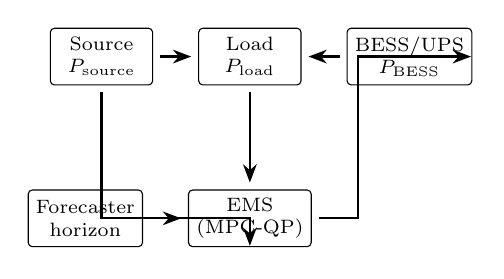
\begin{tikzpicture}[
  >=Stealth,
  box/.style={draw, rounded corners=1.5pt, align=center, inner sep=2.8pt, outer sep=1.2pt, font=\scriptsize},
  arr/.style={->, thick, shorten >=1.5pt, shorten <=1.5pt},
  node distance=0.6cm and 0.5cm
]
\node[box, minimum width=1.3cm, minimum height=0.72cm] (source) {Source\\$P_{\mathrm{source}}$};
\node[box, minimum width=1.3cm, minimum height=0.72cm, right=of source] (load) {Load\\$P_{\mathrm{load}}$};
\node[box, minimum width=1.4cm, minimum height=0.72cm, right=of load] (bess) {BESS/UPS\\$P_{\mathrm{BESS}}$};
\node[box, minimum width=1.3cm, minimum height=0.72cm, below=1.25cm of load] (ems) {EMS\\(MPC-QP)};
\node[box, minimum width=1.3cm, minimum height=0.72cm, left=of ems] (fore) {Forecaster\\horizon};
\draw[arr] (source) -- (load);
\draw[arr] (bess) -- (load);
\draw[arr] (load) -- (ems);
\draw[arr] (fore) -- (ems);
\draw[arr] (source.south) -- ++(0,-1.65) -| (ems.south);
% route to the RIGHT of BESS (not through its center)
\draw[arr] (ems.east) -- ++(0.55,0) |- (bess.east);
\end{tikzpicture}
\caption{Aggregated architecture: source, critical load and BESS/UPS under the EMS-MPC, with a horizon event/load forecaster.}
\label{fig:architecture}
\end{figure}

\begin{table}[!t]
\centering
\caption{Sign convention}
\label{tab:signs}
\begin{tabular}{@{}ll@{}}
\toprule
Symbol & Meaning \\
\midrule
$P_{\mathrm{BESS}}>0$ / $P_{\mathrm{d}}\ge 0$ & Discharge (power to the load) \\
$P_{\mathrm{BESS}}<0$ / $P_{\mathrm{c}}\ge 0$ & Charge (power from the source) \\
$P_{\mathrm{source}}>0$ & Power delivered by the source \\
$P_{\mathrm{unserved}}>0$ & Unserved critical-load power \\
$g=0$ & Source unavailable $\Rightarrow$ $P_{\mathrm{source}}=0$ \\
\bottomrule
\end{tabular}
\end{table}

\subsection{BESS/converter dynamics}
Actual BESS power follows an aggregated first-order model:
\begin{equation}
\label{eq:dyn}
P_{\mathrm{BESS}}(k+1)=a_b\,P_{\mathrm{BESS}}(k)+b_b\,u(k),
\end{equation}
with $u(k)=P_{\mathrm{BESS}}^{\mathrm{ref}}(k)$,
\begin{equation}
a_b=\mathrm{e}^{-T_s/\tau_b},\qquad b_b=1-a_b,
\end{equation}
where $T_s$ is the sampling period and $\tau_b$ is the aggregated converter time constant. After the dynamic update, $P_{\mathrm{BESS}}$ is saturated in $[P_{\mathrm{BESS}}^{\min},P_{\mathrm{BESS}}^{\max}]$ and protected by SOC limits. Inner current/voltage loops, LCL filters, PLL and DC-link transfer are \emph{not} modelled; varying $\tau_b$ does not validate an electrochemical cell or a UPS topology. The load is 100\% critical: no priority classes or shedding.

\subsection{SOC update}
\subsubsection{Simulated plant}
SOC on the plant is updated from the net energy exchanged over $T_s$, converted to a percentage of $E_{\mathrm{bat}}$. Distinct discharge ($\eta_{\mathrm{d}}$) and charge ($\eta_{\mathrm{c}}$) efficiencies are used (both $0.95$ in the case study). With $P_b^{+}\triangleq P_{\mathrm{BESS}}(k+1)$,
\begin{equation}
\label{eq:soc}
\Delta\mathrm{SOC}(k)=
\begin{cases}
\dfrac{P_b^{+}T_s\cdot 100}{3600\,E_{\mathrm{bat}}\,\eta_{\mathrm{d}}}, & P_b^{+}\ge 0,\\[6pt]
\dfrac{P_b^{+}T_s\,\eta_{\mathrm{c}}\cdot 100}{3600\,E_{\mathrm{bat}}}, & P_b^{+}< 0.
\end{cases}
\end{equation}
and
\begin{equation}
\mathrm{SOC}(k+1)=\mathrm{sat}\!\big(\mathrm{SOC}(k)-\Delta\mathrm{SOC}(k),\ \mathrm{SOC}_{\min},\ \mathrm{SOC}_{\max}\big).
\end{equation}

\subsubsection{Internal MPC-QP / myopic QP predictor}
To keep the QP convex and reduce the plant--predictor mismatch on charging, distinct gains
\begin{equation}
K_{\mathrm{d}}=\frac{T_s}{3600\,E_{\mathrm{bat}}\,\eta_{\mathrm{d}}}\cdot 100,\qquad
K_{\mathrm{c}}=\frac{T_s\,\eta_{\mathrm{c}}}{3600\,E_{\mathrm{bat}}}\cdot 100
\end{equation}
are applied by successive linearization. Linearization is performed once per control step (at each sampling instant $k$), when the QP is assembled, and is recomputed every sample from the measured/plant power $P_{\mathrm{BESS}}(k)$ and the free-response trajectory $P_{\mathrm{BESS}}^{\mathrm{free}}$ over the horizon---the open-loop response under the previous reference held constant, with no dependence on the previous QP solution for the sign choice. At each predicted step $i$, the sign of $P_{\mathrm{BESS},i}^{\mathrm{free}}$ selects the $K_{\mathrm{d}}$ (discharge) or $K_{\mathrm{c}}$ (charge) branch; with these gains fixed, the SOC map remains linear in the decision variables, so the QP remains convex. This removes the systematic $\approx 1/\eta^2$ charging error of a single-gain predictor without increasing the QP dimension. The plant continues to apply~\eqref{eq:soc} with saturations.

\subsection{Case-study parameters}
Nominal parameters are summarized in Table~\ref{tab:param}. QP weights (Table~\ref{tab:weights}) impose an approximate priority hierarchy via normalized magnitudes: load supply and event support dominate source tracking, SOC, ramps and BESS usage.

\begin{table*}[!t]
\centering
\caption{Nominal case-study parameters}
\label{tab:param}
{\footnotesize\setlength{\tabcolsep}{6pt}%
\begin{tabular}{@{}llc@{}}
\toprule
Symbol / item & Description & Value \\
\midrule
$T_s$ & Sampling period & \SI{1}{\second} \\
$T_f$ & Short simulation horizon & \SI{1200}{\second} \\
$\tau_b$ & Converter time constant & \SI{2}{\second} \\
$E_{\mathrm{bat}}$ & BESS energy capacity & \SI{500}{\kilo\watt\hour} \\
$P_{\mathrm{BESS}}^{\max}$ & Maximum discharge & \SI{400}{\kilo\watt} \\
$P_{\mathrm{BESS}}^{\min}$ & Maximum charge (negative) & \SI{-250}{\kilo\watt} \\
$P_{\mathrm{source}}^{\max,\mathrm{nom}}$ & Nominal source limit & \SI{800}{\kilo\watt} \\
$R_{\mathrm{source}}^{\max}$ & Desired source ramp & \SI{100}{\kilo\watt\per\second} \\
Typical $P_{\mathrm{load}}$ & Base / medium / high & 600 / 750 / 950\,kW \\
$\mathrm{SOC}_{\min}/\mathrm{SOC}_{\mathrm{ref}}/\mathrm{SOC}_{\max}$ & Limits and reference & 20 / 60 / 90\,\% \\
$\eta_{\mathrm{d}},\eta_{\mathrm{c}}$ & Charge/discharge efficiencies & 0.95 \\
$N_p$, $N_c$ & Prediction/control horizons & 60 / 15 \\
$N_{\mathrm{prep}}$ & Event-preparation window & 30 steps \\
$\Delta u_{\max}$ & $u$ rate limit (normal/event) & 120 / 400\,kW \\
\bottomrule
\end{tabular}}
\end{table*}

\begin{table}[!t]
\centering
\caption{Nominal QP weights (terms normalized by $P_{\mathrm{base}}$, $R_{\mathrm{base}}$ or $100\,\%$)}
\label{tab:weights}
\begin{tabular}{@{}llc@{}}
\toprule
Weight & Term & Value \\
\midrule
$w_L$ & Load slack $S_{\mathrm{load}}$ & $10^{9}$ \\
$w_E$ & Event slack $S_{\mathrm{event}}$ & $10^{9}$ \\
$w_G$ & Source slack $S_{\mathrm{source}}$ & $10^{8}$ \\
$w_C$ & Recharge slack $S_{\mathrm{rech}}$ & $10^{6}$ \\
$w_P$ & Source tracking & $3\cdot 10^{3}$ \\
$w_S$ / $w_T$ & SOC horizon / terminal & $1.2\cdot 10^{3}$ / $1.2\cdot 10^{4}$ \\
$w_R$ & Source ramp & $300$ \\
$w_B$ & BESS usage & $20$ \\
$w_{\Delta u}$ & $\Delta u$ variation & $50$ \\
\bottomrule
\end{tabular}
\end{table}

\section{Control Strategies}
\label{sec:control}

Each controller answers a distinct design question (Table~\ref{tab:baseline_role}): the heuristic measures the performance of a simple reactive operating rule; Heur+FS measures how much is gained from future information alone, without multi-step optimization; the myopic QP measures how much is gained from constrained optimization without a future horizon; FF+FB (later package) measures a non-QP law with the same forecasts; MPC-QP measures the combined effect of foresight, a dynamic model and multi-step optimization. The 11~September comparison isolates forecast versus optimization under the same plant; FF+FB is labelled separately.

\begin{table}[!t]
\centering
\caption{Role of each baseline in the comparison (FS: foresight; Hor.: horizon)}
\label{tab:baseline_role}
{\footnotesize\setlength{\tabcolsep}{2.5pt}%
\begin{tabular}{@{}lcccc@{}}
\toprule
Controller & FS? & QP? & Hor.? & Role \\
\midrule
Heuristic & No & No & No & reactive \\
Heur+FS & Yes & No & Partial & forecast effect \\
Myopic QP & No & Yes & No & local QP \\
MPC-QP (V5) & Yes & Yes & Yes & proposed deterministic \\
Stochastic 3-sc. & Yes & Yes & Yes & tail / reserve cost \\
FF+FB (later) & Yes & No & No & same forecasts, no QP \\
\bottomrule
\end{tabular}}
\end{table}

\subsection{Heuristic controller}
The heuristic implements supervisory rules:
\begin{itemize}
\item if $g(k)=0$, then $u(k)=\min\!\big(P_{\mathrm{load}}(k),P_{\mathrm{BESS}}^{\max}\big)$;
\item if $P_{\mathrm{load}}(k)>P_{\mathrm{source}}^{\max}(k)$, the BESS covers the deficit;
\item if source headroom exists and $\mathrm{SOC}<\mathrm{SOC}_{\mathrm{ref}}$, the BESS recharges up to a charge-power limit;
\item otherwise, $u(k)=0$.
\end{itemize}
This baseline is interpretable and strictly reactive (no forecast). Alternative heuristic tunings (different charge-power caps or emergency $\Delta u$) were not exhaustively re-optimized; the fairness campaign instead equalizes the \emph{common} $\Delta u_{\max}$ knob across QP controllers. A shared ramp limit does not equalize costs, supervision or emergency policy.

\subsection{Heuristic with foresight (Heur+FS)}
To isolate the value of prediction, a foresight-enabled heuristic (Heur+FS) receives the \emph{same} future load, limit and $g$ window as the MPC-QP ($N_{\mathrm{prep}}$). Before a detected event it applies a proximity-proportional preparation ramp; at contingency onset it uses the same reactive rules. It does not solve a QP, thus comparing forecast + rules versus forecast + multi-step optimization.

\subsection{Myopic QP (one-step optimization)}
At each $k$, the myopic QP solves a QP for the current instant only:
\begin{equation}
z=\big[u,\ P_{\mathrm{grid}},\ s_{\mathrm{load}},\ s_{\mathrm{source}},\ s_{\mathrm{rech}}\big]^\top.
\end{equation}
One-step BESS power is predicted by~\eqref{eq:dyn} and the balance
\begin{equation}
P_{\mathrm{grid}}+P_{\mathrm{BESS}}(k+1)+s_{\mathrm{load}}=P_{\mathrm{load}}(k)
\end{equation}
is imposed, together with power/SOC limits (gains $K_{\mathrm{d}}/K_{\mathrm{c}}$), source tracking, ramps and $u$ rate limits. There is no horizon and no event preparation.

\subsection{Feedforward plus feedback (later package)}
\label{sec:ff}
FF+FB is \emph{not} a proportional SOC-error law. It uses the same event/recharge supervisor as the audited assembler (\texttt{referencias\_evento\_v2}) and inverts the first-order converter map on the current sample. With source reference $P_{\mathrm{source},k}^{\mathrm{ref}}$ from that supervisor,
\begin{equation}
r_k=P_{\mathrm{load}}(k)-P_{\mathrm{source},k}^{\mathrm{ref}},\qquad
u_k^{\star}=(r_k-a_b P_{\mathrm{BESS}}(k))/b_b.
\end{equation}
SOC then only \emph{blocks} infeasible signs ($u{=}0$ if $\mathrm{SOC}\le\mathrm{SOC}_{\min}$ and $u^{\star}{>}0$, or $\mathrm{SOC}\ge\mathrm{SOC}_{\max}$ and $u^{\star}{<}0$); recharge enablement is a threshold on SOC versus $\mathrm{SOC}_{\mathrm{ref}}$ minus a deadband, not a $K_p$ term. After $g(k){=}0\Rightarrow u\ge 0$, the command is saturated to $[P_{\mathrm{BESS}}^{\min},P_{\mathrm{BESS}}^{\max}]$ and to $|u-u_{k-1}|\le \Delta u_{\max}$ (event versus normal rate). Package B2 uses persistence fill of future $g$; the 11~September V5 jobs use return-to-normal fill. Table~\ref{tab:ff} reports B2 jobs \texttt{B2\_ff\_0001}/\texttt{B2\_ff\_0003} against 11~September V5 jobs \texttt{j00004}/\texttt{j00014}. It is not a sixth column of Table~\ref{tab:punserved} and is not a validated official campaign (\texttt{ready\_for\_article=false}).

\subsection{Event-anticipating MPC-QP}
\label{sec:mpc}
MPC-QP optimizes $\Delta u$ over $N_c$ with prediction over $N_p$. The decision vector is
\begin{equation}
z=\big[\Delta U;\ P_{\mathrm{grid}};\ S_{\mathrm{load}};\ S_{\mathrm{source}};\ S_{\mathrm{rech}};\ S_{\mathrm{event}}\big],
\end{equation}
with dimension $N_c+5N_p$ (nominally $15+5\cdot 60=315$). BESS references reconstruct as
\begin{equation}
u_{k+i|k}=u(k-1)+\sum_{j=0}^{\min(i,N_c-1)}\Delta u_{k+j|k}.
\end{equation}
$P_{\mathrm{BESS}}$ follows~\eqref{eq:dyn}; predicted SOC uses $K_{\mathrm{d}}/K_{\mathrm{c}}$ by successive linearization. Predictive balance is
\begin{equation}
P_{\mathrm{grid},i}+P_{\mathrm{BESS},i}+S_{\mathrm{load},i}=P_{\mathrm{load},i},
\end{equation}
with $g_i=0\Rightarrow P_{\mathrm{grid},i}=0$.

\subsubsection{Event detection and minimum support}
Define $\delta_i=\max(P_{\mathrm{load},i}-P_{\mathrm{source},i}^{\max},0)$ and
\begin{equation}
\label{eq:support}
P_{\mathrm{BESS},i}^{\min,\mathrm{evt}}=
\begin{cases}
\min\!\big(P_{\mathrm{load},i},P_{\mathrm{BESS}}^{\max}\big), & g_i=0,\\[2pt]
\min\!\big(\delta_i,P_{\mathrm{BESS}}^{\max}\big), & \delta_i>0,\\[2pt]
0, & \text{o.w.}
\end{cases}
\end{equation}
A preparation ramp over $N_{\mathrm{prep}}$ precedes the first event; this window only shapes pre-actuation/tracking, while primary foresight comes from the horizon $N_p$ and the event constraint~\eqref{eq:event}. The soft constraint is
\begin{equation}
\label{eq:event}
P_{\mathrm{BESS},i}+S_{\mathrm{event},i}\ge P_{\mathrm{BESS},i}^{\min,\mathrm{evt}}.
\end{equation}

\subsubsection{Cost function}
With normalized variables,
\begin{equation}
\label{eq:cost}
\begin{aligned}
J &= w_L\|\tilde{S}_{\mathrm{load}}\|^2
 + w_G\|\tilde{S}_{\mathrm{source}}\|^2
 + w_E\|\tilde{S}_{\mathrm{event}}\|^2 \\
&\quad
 + w_P\|\tilde{P}_{\mathrm{grid}}-\tilde{P}_{\mathrm{ref}}\|^2 \\
&\quad
 + w_S\|\tilde{\mathrm{SOC}}-\tilde{\mathrm{SOC}}_{\mathrm{ref}}\|^2 \\
&\quad
 + w_T(\tilde{\mathrm{SOC}}_{N_p}-\tilde{\mathrm{SOC}}_{\mathrm{ref}})^2 \\
&\quad
 + w_R\|\Delta\tilde{P}_{\mathrm{grid}}\|^2
 + w_B\|\tilde{P}_{\mathrm{BESS}}\|^2 \\
&\quad
 + w_{\Delta u}\|\Delta U\|^2
 + w_C\|\tilde{S}_{\mathrm{rech}}\|^2.
\end{aligned}
\end{equation}
The terminal term is an SOC cost only; it is not a terminal set nor a formal stability certificate.

\subsubsection{Implementation}
We use $N_p=60$, $N_c=15$, $N_{\mathrm{prep}}=30$, $T_s=\SI{1}{\second}$ for the golden V5. Audited QPs are normalized with $P_{\mathrm{base}}=\SI{950}{\kilo\watt}$ and $R_{\mathrm{base}}=\SI{100}{\kilo\watt\per\second}$ (the historical V5 builder used a trajectory-dependent base; the myopic used instantaneous bases---the revision campaign freezes the audited pair). The QP is solved with MATLAB \texttt{quadprog} (\texttt{interior-point-convex}) and constraint preallocation. The audited \texttt{quadprog} call passes an empty $X_0$; a dedicated warm-start trial reproduced the same iteration counts and solutions. Warm-start acceleration is therefore \emph{not} used and is not claimed. Solver failures trigger a heuristic fallback classified by \texttt{exitflag}; fallback is part of the closed-loop policy and is reported, not hidden. A candidate Hessian rescaling of the IPM did not pass a pre-registered KKT gate (13/15 cases); official numbers remain the 11~September consolidation.

\subsection{Three-scenario stochastic MPC}
The fifth competitor is a scenario MPC built in this project: three internal trajectories (nominal forecast, future load ${+}20\%$, interruption announced \SI{10}{\second} early) with equal probabilities, a \emph{shared} command sequence $\Delta U$, and scenario-specific predicted states and slacks. The whole $\Delta U$ is shared across scenarios; only the first increment is applied and the remainder is discarded at the next sample. Identical scenarios are merged by adding probabilities. This is not a claim of multi-stage recourse or of reproducing a named literature policy. Without an announced event, the early-interruption scenario coincides with the nominal one. Sensitivity with probabilities $0.50/0.25/0.25$ is reported as secondary.

The SIL object in Section~\ref{sec:embedded} is \texttt{backend=matlab\_fpga}: a reduced-horizon MATLAB copy ($N_p{=}12$, $N_c{=}4$) that still calls \texttt{controle\_mpc\_qp\_v5} / \texttt{quadprog} in-process. It is not ADMM~C and does \emph{not} send or parse UART frames. The Nios ADMM firmware is a third object: ASCII UART on the board, different solver, demonstrated until OpenCore Plus expired, not a 1200-step KPI table.

\section{Scenarios, Metrics, and Protocol}
\label{sec:scenarios}

Short scenarios ($T_f=\SI{1200}{\second}$, $N=1201$ stored states, metrics integrated over 1200 intervals) share one physical trajectory per named case. The current sample is measured; the future in the horizon is a forecast. For events without an announcement, no controller is given the future interruption. Detection delay is a separate assay. Physical order: measure at $k$, command at $k$, BESS power at $k{+}1$, then balance and SOC. Zero unserved power at $T_s=\SI{1}{\second}$ does not prove sub-second electrical continuity.

Peaks are reported raw and, where stated, filtered with threshold $\max(\SI{1}{\kilo\watt},0.1\%$ of max load). Recovery is defined per event as \SI{10}{\second} sustained below \SI{1}{\kilo\watt}. Filtered zero is not mathematical zero.

\subsection{Group A --- Nominal AI/HPC operation}
Target: eliminate transient $P_{\mathrm{unserved}}$ under demand variation (no grid outage).
\begin{enumerate}
\item \textbf{Load bands:} $P_{\mathrm{load}}$ switches among 600, 750, 950, 700 and 600\,kW.
\item \textbf{Source limit:} load rises from 750 to 950\,kW with $P_{\mathrm{source}}^{\max}=800$\,kW. Without BESS, the structural deficit would be $950-800=\SI{150}{\kilo\watt}$ (analytical no-EMS/$u=0$ reference).
\item \textbf{Multi-burst:} synthetic AI/HPC burst profile with the grid available ($g(k)=1$): medium steps, nearby peaks and light oscillation (Table~\ref{tab:multiburst}). It does not require a grid outage to evidence BESS pre-positioning before load bursts.
\end{enumerate}
Success criteria (Group~A): filtered $P_{\mathrm{unserved}}^{\max}$ below the reporting threshold, small $E_{\mathrm{unserved}}$, no structural source shortfall beyond what the BESS covers, acceptable SOC.

Public traces complement the synthetic steps; they are \emph{not} feeder measurements of a facility owned by the authors. DIPLOEE-derived profiles are simulated facility power (minute native sampling, resampled). NVML profiles are measured GPU power from 16 nodes, aggregated/interpolated and affinely mapped into the 600--950\,kW band. Unit errata: the preparation script stores NVML extrema in fields named \texttt{raw\_min\_W}/\texttt{raw\_max\_W} \emph{after} converting W$\to$kW, so those metadata labels are wrong; the mapped 600--950\,kW traces used in the campaign are unaffected. Twenty registered windows overlap; they are not 20 independent sites. Stress windows were selected for largest amplitude on the \emph{native} traces; each window was then affinely mapped into 600--950\,kW. Amplitude after mapping is therefore not the selection criterion. GPU utilization is not synchronized to a whole-facility feeder in this study.

\begin{table}[!t]
\centering
\caption{Multi-burst profile (intervals and $P_{\mathrm{load}}$ levels; base \SI{600}{\kilo\watt})}
\label{tab:multiburst}
\begin{tabular}{@{}llc@{}}
\toprule
Interval [s] & Level [kW] & Type \\
\midrule
$[120,180)$ & 750 & medium step \\
$[220,260)$ & 950 & short peak \\
$[260,320)$ & 700 & partial recovery \\
$[340,400)$ & 950 & nearby peak \\
$[450,600)$ & 750 & sustained step \\
$[700,780)$ & 950 & final peak \\
$[800,1000)$ & $600+40\sin(\cdot)$ & light oscillation \\
\bottomrule
\end{tabular}
\end{table}

\subsection{Group B --- Short contingencies}
Complementary target: approach the \emph{scenario-specific power bound} $\max(P_{\mathrm{load}}-P_{\mathrm{BESS}}^{\max},0)$ (zero $P_{\mathrm{unserved}}$ is infeasible when $P_{\mathrm{load}}>P_{\mathrm{BESS}}^{\max}$).
\begin{enumerate}
\item \textbf{Source loss:} constant 750\,kW; $g(k)=0$ on $[500,650)$\,s.
\item \textbf{Source return:} outage on $[400,650)$\,s with later restoration.
\end{enumerate}
Success criteria (Group~B): $P_{\mathrm{unserved}}^{\max}$ near that bound; $E_{\mathrm{unserved}}$ dominated by BESS power limit; SOC above $\mathrm{SOC}_{\min}$; low fallback.

\subsection{Group C --- Energy bound}
Prolonged critical outage ($\approx\SI{2}{\hour}$): demonstrate that finite energy dominates the outcome; avoid overclaiming continuity.

\subsection{Information policy}
\label{sec:infopol}
Current measurements at $k$ are common to every controller. Future load, source limit and $g$ in the horizon are forecasts. Scheduled load steps, planned interruptions and protection alarms are distinct cues; an unannounced outage hides future $g$ from all compared policies. Detection delay is a separate assay and is not a draw from the Monte Carlo delay law.

When foresight of $g$ is off, the 11~September assembler still fills future source-available / nominal limit into the QP: a causal return-to-normal hypothesis, not persistence of the measured outage. Package B2/B6 used for FF+FB and the second-event test instead fills persistence of the measured outage. Both fills are declared; neither is a field-identified detector. A feedforward-plus-feedback competitor with the same supervisor \emph{was} run as package B2 (Section~\ref{sec:ff}); it is not in Table~\ref{tab:punserved}.

SOC inequality uses the tabulated $\mathrm{SOC}_{\min}$ with zero extra margin in the audited maps. Weights in Table~\ref{tab:weights} were chosen so that load/event slacks dominate after $P_{\mathrm{base}}$ normalization; a univariate $\times 0.5/1/2$ sweep on five V5 weights in two scenarios did not reverse the Group~A ranking, but it does not cover source-tracking, ramp, SOC, terminal and BESS-usage jointly, nor myopic-specific weights. Large slacks are an \emph{approximate} priority, not lexicographic MPC. The reported constraint-gram indicator is $\mathrm{condest}(C^\top C+\varepsilon I)$ at the first step, not the condition of $C$ itself.

The nominal case assumes known horizon profiles (perfect foresight in the baseline). Additional tests inject magnitude errors ($\pm 10\%$, $\pm 20\%$) and a dense timing grid on $[-20,+20]$\,s into the forecast seen by MPC.

\subsection{Additional studies}
\begin{itemize}
\item Foresight ON/OFF and foresight-enabled heuristic (Heur+FS).
\item Sensitivity to $N_{\mathrm{prep}}$ and $\tau_b$.
\item Forecast-error sweeps (magnitude and timing) and a 200-pair Monte Carlo (Normal delays clipped to $\pm\SI{20}{\second}$, $\sigma=\SI{6}{\second}$, load error uniform on $[-20\%,+20\%]$), with the \emph{same} physical outage and different forecast errors---not a population of data centers.
\item Fairness on the myopic $\Delta u$ limit and isolated ablations (foresight off, unit horizon, event inequality).
\item MATLAB SIL ($N_p{=}12$, \texttt{quadprog}) and UART HIL of the heuristic (Section~\ref{sec:embedded}).
\end{itemize}

\subsection{Metrics}
We report $P_{\mathrm{unserved}}^{\max}$, unserved energy $E_{\mathrm{unserved}}$, duration $T_{\mathrm{unserved}}$, SOC (final/min/at event), throughput and equivalent full cycles $N_{\mathrm{EFC}}$ (a utilization proxy, not a lifetime model), maximum source ramp, fallback percentage and QP timings. Table~\ref{tab:tqp} uses \emph{median} and max $t_{\mathrm{QP}}$ from the 11~September CSV; Table~\ref{tab:nprep} reports historical \emph{mean} $t_{\mathrm{QP}}$ and is labelled as such. Preparation-energy, reversal-count and \texttt{aging\_proxy} fields exist in later packages but are not paper KPIs: \texttt{aging\_proxy} is a multiple of throughput, and the preparation/reversal definitions are not the quantities requested by the reviewers. For contingencies we also use distance to the scenario-specific bound $P_{\mathrm{unserved}}^{\max}-(P_{\mathrm{load}}-P_{\mathrm{BESS}}^{\max})$. For load variation we report transient reduction relative to the heuristic $(P_{\mathrm{unserved},\mathrm{heur}}^{\max}-P_{\mathrm{unserved}}^{\max})/P_{\mathrm{unserved},\mathrm{heur}}^{\max}$. Under outages, the maximum source ramp includes the exogenous drop induced by $g(k)$ and must not be read as a voluntary EMS operating ramp. Equal heuristic peaks on load-bands and source-limit ($90.979599$\,kW) are not a copy-paste error: both expose a $150$\,kW first-step deficit through $\tau_b=\SI{2}{\second}$, $150\,\mathrm{e}^{-1/2}=90.979599$\,kW, at different event times ($400$\,s vs.\ $200$\,s).

\section{Results and Discussion}
\label{sec:results}
\FloatBarrier

The results are interpreted under two different objectives. In load-variation scenarios (Group~A), the target is to eliminate transient unserved power (filtered). In contingency scenarios (Group~B), the target is not zero---infeasible when $P_{\mathrm{load}}>P_{\mathrm{BESS}}^{\max}$---but to approach the scenario-specific bound $P_{\mathrm{load}}-P_{\mathrm{BESS}}^{\max}=\SI{350}{\kilo\watt}$ at \SI{750}{\kilo\watt} load. Desktop numbers below are the 11~September consolidation unless noted.

\subsection{Main comparison}
Table~\ref{tab:punserved} summarizes $P_{\mathrm{unserved}}^{\max}$ across all short scenarios and shows these two regimes: in load-variation regimes, the performance target is zero unserved power, and MPC-QP reaches it; in source-contingency regimes, the performance target is not zero, but the scenario-specific bound, which MPC-QP reaches when foresight is adequate. In the nominal load-bands and source-limit cases, MPC-QP removes the \emph{filtered} transient residual ($0$\,kW; raw V5 load-band peak $0.018$\,kW), whereas heuristic and myopic QP exhibit peaks of about \SIrange{91}{103}{\kilo\watt} linked to~\eqref{eq:dyn}. On multi-burst the myopic peak is $108.90$\,kW. Relative to the heuristic, transient reduction is $100\,\%$ for MPC-QP and $\approx 94.9\,\%$ for Heur+FS (load bands / source limit). Heur+FS improves the step transient when the demand change is anticipable, but without multi-step optimization it typically does not match MPC-QP. This gain is the most relevant for AI data centers, because demand steps and contractual-limit saturation are recurring---not exceptional---operating events. Table~\ref{tab:metrics} complements with $E_{\mathrm{unserved}}$, final SOC and fallback on the two key scenarios.

Under contingencies (complementary study), heuristic and myopic QP reach $\approx\SI{593}{\kilo\watt}$, consistent with the first step from $P_{\mathrm{BESS}}\approx 0$ and $u=P_{\mathrm{BESS}}^{\max}$:
\begin{align}
P_{\mathrm{BESS}}^{+}
&\approx b_b\cdot 400
\approx\SI{157}{\kilo\watt},\\
P_{\mathrm{unserved}}
&\approx 750-157
=\SI{593}{\kilo\watt}.
\end{align}
With anticipation, MPC-QP arrives at the outage already near \SI{400}{\kilo\watt}, reducing $P_{\mathrm{unserved}}^{\max}$ to the scenario-specific bound
\begin{equation}
P_{\mathrm{unserved}}^{\mathrm{floor}}=P_{\mathrm{load}}-P_{\mathrm{BESS}}^{\max}=\SI{350}{\kilo\watt}.
\end{equation}
Distance to that bound on source loss is $242.61$\,kW (heuristic), $12.47$\,kW (Heur+FS) and $\approx 0.07$\,kW (MPC-QP V5). Heur+FS is near the bound on a single contingency ($362.47$ vs.\ $350.07$\,kW) but fails on multi-burst ($60.65$ vs.\ filtered $0$\,kW): simple foresight helps for an isolated event, whereas multi-step optimization becomes decisive when several events and SOC/ramp trade-offs interact. This bound is not a controller failure: it is $P_{\mathrm{load}}-P_{\mathrm{BESS}}^{\max}$ for this rating pair. Over $150$\,s at $350$\,kW the persistent energy floor is $14.5833$\,kWh. Even an optimal EMS cannot invent energy or power beyond the available storage.

\begin{table*}[!t]
\centering
\caption{Raw $P_{\mathrm{unserved}}^{\max}$ [kW], 11~September campaign (filter threshold \SI{1}{\kilo\watt}: MPC-QP V5 load-band/limit/multi-burst/NVML/DIPLOEE filtered peaks are 0)}
\label{tab:punserved}
{\footnotesize
\begin{tabular}{@{}lccccc@{}}
\toprule
Scenario & Heur. & Heur+FS & Myopic & MPC-QP V5 & Stoch.\ 3-sc. \\
\midrule
Load bands & 90.98 & 4.67 & 102.78 & 0.018 & $\approx 0$ \\
Source limit & 90.98 & 4.67 & 102.78 & $\approx 0$ & $\approx 0$ \\
Multi-burst & 90.98 & 60.65 & 108.90 & 0.018 & $\approx 0$ \\
DIPLOEE stress & 2.67 & 2.67 & $\approx 0$ & 0.002 & $\approx 0$ \\
NVML stress & 52.73 & 48.51 & 28.37 & 0.007 & $\approx 0$ \\
Source loss & 592.61 & 362.47 & 592.61 & 350.07 & 350.00 \\
Source return & 592.61 & 362.47 & 592.61 & 350.09 & 350.00 \\
\bottomrule
\end{tabular}}
\end{table*}

\begin{table}[!t]
\centering
\caption{Complementary metrics: load bands and source loss}
\label{tab:metrics}
\begin{tabular}{@{}llcccc@{}}
\toprule
Scenario & Control & $P_{\mathrm{unserved}}^{\max}$ & $E_{\mathrm{unserved}}$ & SOC$_f$ & FB \\
 &  & [kW] & [kWh] & [\%] & [\%] \\
\midrule
Load bands & Heuristic & 90.98 & 0.064 & 59.51 & 0 \\
Load bands & Heur+FS & 4.67 & 0.003 & 59.52 & 0 \\
Load bands & Myopic QP & 102.78 & 0.036 & 59.25 & 0 \\
Load bands & MPC-QP V5 & 0.018$^{\dagger}$ & $\approx 0$ & 58.80 & 0 \\
Load bands & Stoch.\ 3-sc. & $\approx 0$ & $\approx 0$ & 53.36 & 0 \\
Source loss & Heuristic & 592.61 & 14.75 & 57.94 & 0 \\
Source loss & Heur+FS & 362.47 & 14.59 & 57.54 & 0 \\
Source loss & Myopic QP & 592.61 & 14.75 & 57.91 & 0 \\
Source loss & MPC-QP V5 & 350.07 & 14.58 & 57.10 & 1.58 \\
Source loss & Stoch.\ 3-sc. & 350.00 & 14.58 & 49.40 & 0 \\
\bottomrule
\end{tabular}
\end{table}
{\scriptsize $^{\dagger}$Raw peak; filtered value is 0 at the \SI{1}{\kilo\watt} threshold.}

Table~\ref{tab:metrics} shows that MPC-QP does not win on peak alone: on load bands it drives filtered $E_{\mathrm{unserved}}$ to $0$\,kWh (vs.\ $0.064$\,kWh for the heuristic) with final SOC $58.80\,\%$ vs.\ $59.51\,\%$. The stochastic competitor matches the filtered peak at a larger SOC spend ($53.36\,\%$) and roughly double throughput---a reserve cost, not a free lunch. On source loss, V5 reduces the peak to $350.07$\,kW ($\approx 40.9\%$ vs.\ the heuristic) with energy $14.58$ vs.\ $14.75$\,kWh ($\approx 1.16\%$ energy cut) and $1.58\%$ fallback; the stochastic copy sits on $350.00$\,kW with SOC $49.40\,\%$. Filtered zero in Group~A is not obtained by oversizing the source: at the source-limit step, $P_{\mathrm{source}}^{\max}$ remains $800$\,kW while the load reaches $950$\,kW (structural deficit without BESS $\approx\SI{150}{\kilo\watt}$). Across 20 NVML windows, mean unserved energy is $6.321$\,kWh (heuristic), $3.134$\,kWh (myopic) and $<10^{-3}$\,kWh for both MPCs; occasional raw MPC peaks of a few kilowatts occur on the first sample.

Fairness: raising the myopic $\Delta u_{\max}$ from 120 to 200 to $400$\,kW/s on the source-limit case yields $102.78$, $71.31$ and $\approx 0$\,kW. Horizon is therefore not necessary for a near-zero peak in that isolated knob test. The myopic penalty is $w_{\Delta u}(u-u_{\mathrm{prev}})^2/P_{\mathrm{base}}^2$ whereas V5 uses $w_{\Delta u}\|\Delta U\|^2$ \emph{without} that $P_{\mathrm{base}}$ division ($P_{\mathrm{base}}=950$\,kW, $w_{\Delta u}=50$ $\Rightarrow$ coefficient ratio on the order of $9\times 10^{5}$ in normal mode). Equal weight \emph{names} do not equalize costs; the closest horizon ablation is V5 with $N_c=N_p=1$, not the separate myopic controller. With $\Delta u_{\max}=400$\,kW/s, multi-burst and NVML still favor MPC. Isolated removal of the event inequality changes source-loss V5 only from $350.067$ to $350.129$\,kW---keep the constraint, but do not call it the main gain. Without future preview, V5 source-loss returns to $592.56$\,kW. When foresight of $g$ is off, the audited assembler still writes future source-available / nominal limit into the QP (a causal ``return-to-normal'' hypothesis, not persistence of the measured outage).

Table~\ref{tab:ff} shows that FF+FB already drives the load-band filtered peak to zero (throughput $18.71$ vs.\ V5 $19.86$\,kWh; SOC$_f$ $59.11\%$ vs.\ $58.80\%$) and a source-loss peak of $355.95$\,kW versus V5 $350.07$\,kW (energy $14.59$ vs.\ $14.58$\,kWh). On this plant, multi-step QP is therefore \emph{not} uniquely necessary for the Group~A zeros; V5 still sits closer to the $350$\,kW physics bound on source loss.

\begin{table}[!t]
\centering
\caption{FF+FB (B2, persistence: \texttt{B2\_ff\_0001}/\texttt{B2\_ff\_0003}) versus V5 (11~Sep: \texttt{j00004}/\texttt{j00014})}
\label{tab:ff}
{\footnotesize\setlength{\tabcolsep}{3pt}%
\begin{tabular}{@{}lcccc@{}}
\toprule
Scenario & FF $P_{\mathrm{un}}^{\max}$ & V5 $P_{\mathrm{un}}^{\max}$ & FF SOC$_f$ & V5 SOC$_f$ \\
 & [kW] & [kW] & [\%] & [\%] \\
\midrule
Load bands & $\approx 0$ & 0.018 & 59.11 & 58.80 \\
Source loss & 355.95 & 350.07 & 57.52 & 57.10 \\
\bottomrule
\end{tabular}}
\end{table}

Fig.~\ref{fig:load_panels} shows the full comparison for the load-band scenario---the primary evidence of the contribution. MPC-QP anticipates demand steps, reducing $P_{\mathrm{unserved}}$ transients and coordinating $P_{\mathrm{BESS}}$ and SOC more effectively than strategies without a horizon.

\begin{figure*}[!t]
\centering
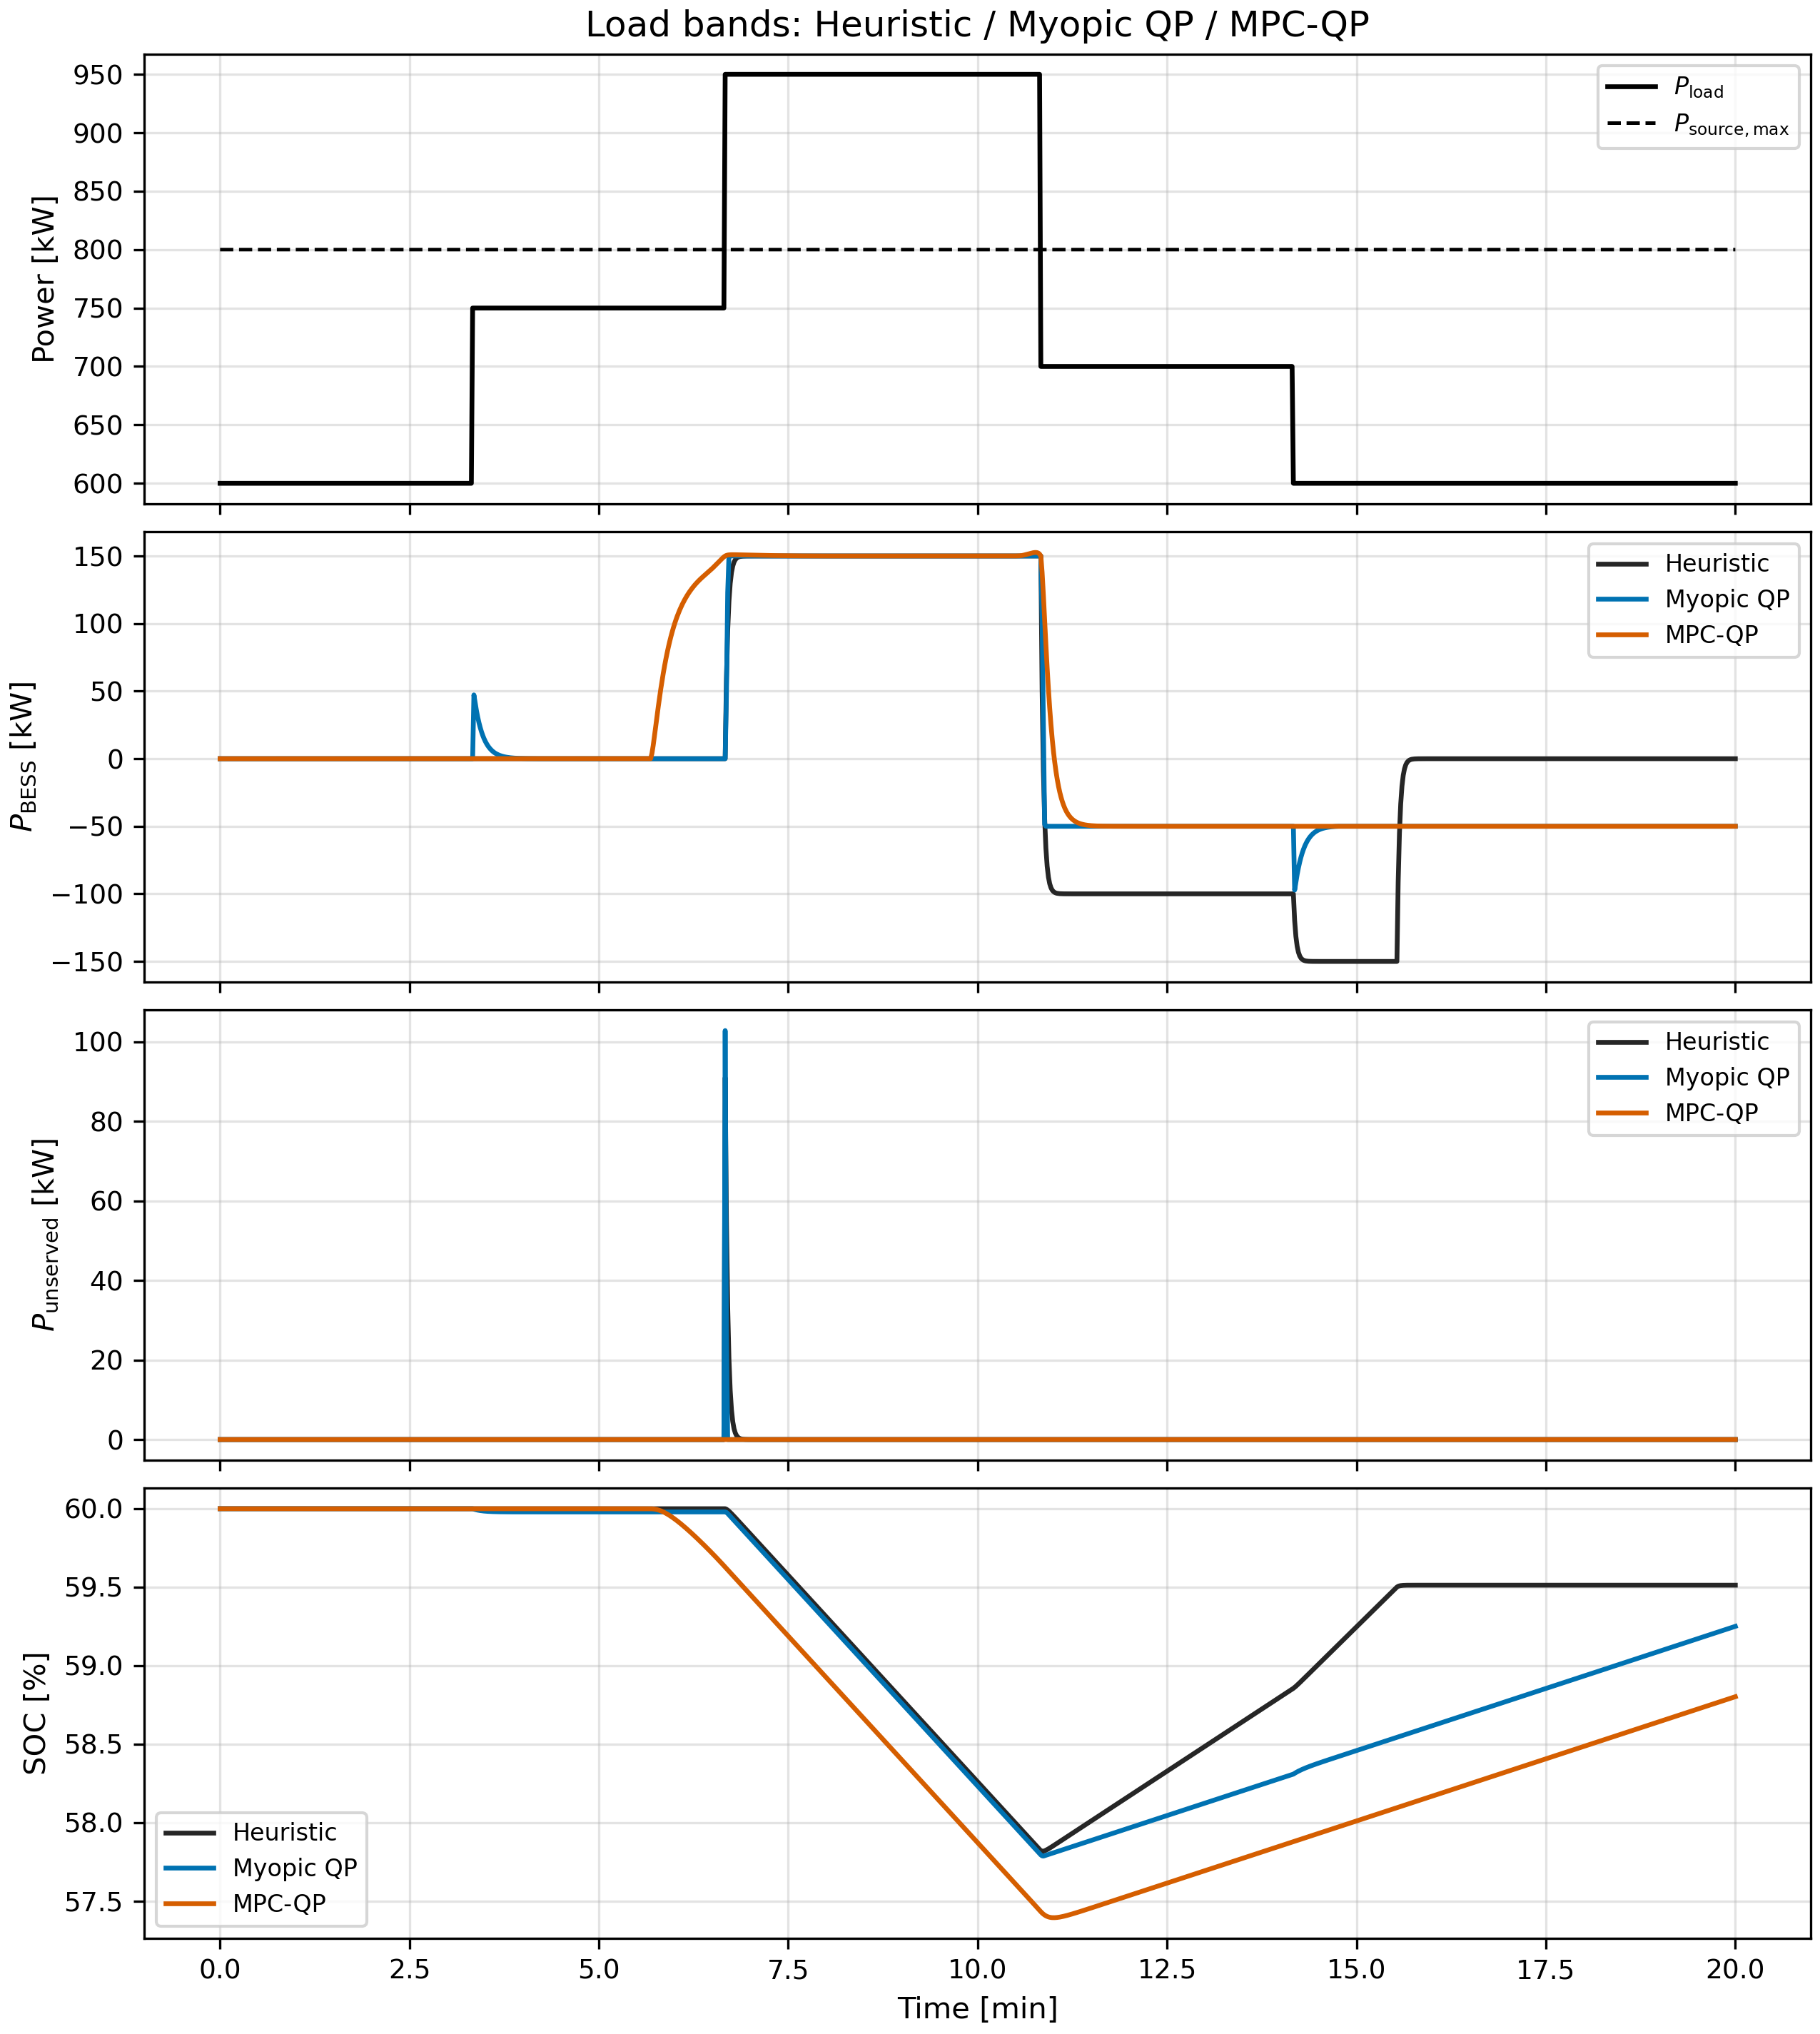
\includegraphics[width=0.85\textwidth]{comp_carga_faixas_paineis.png}
\caption{Load bands, 11~September campaign (jobs \texttt{j00001}/\texttt{j00003}/\texttt{j00004}): heuristic, myopic QP and MPC-QP---load, source, BESS, SOC and unserved power.}
\label{fig:load_panels}
\end{figure*}

Fig.~\ref{fig:limit_zoom} reinforces the same point in the source-limit scenario (step zoom; full panels omitted for space). At the $750\to 950$\,kW step, MPC-QP pre-positions the BESS and keeps $P_{\mathrm{unserved}}=0$; the heuristic exhibits a peak of $\approx\SI{90.98}{\kilo\watt}$. The myopic QP, although locally optimal, is worse than the heuristic in this transient ($\approx\SI{102.78}{\kilo\watt}$ vs.\ $\approx\SI{90.98}{\kilo\watt}$): with $\Delta u$ rate limits, ramp/SOC/$\Delta u$ penalties and no future-step visibility, it does not pre-position the BESS and tends to react more conservatively than the heuristic rule, which jumps harder on the deficit.

\begin{figure*}[!t]
\centering
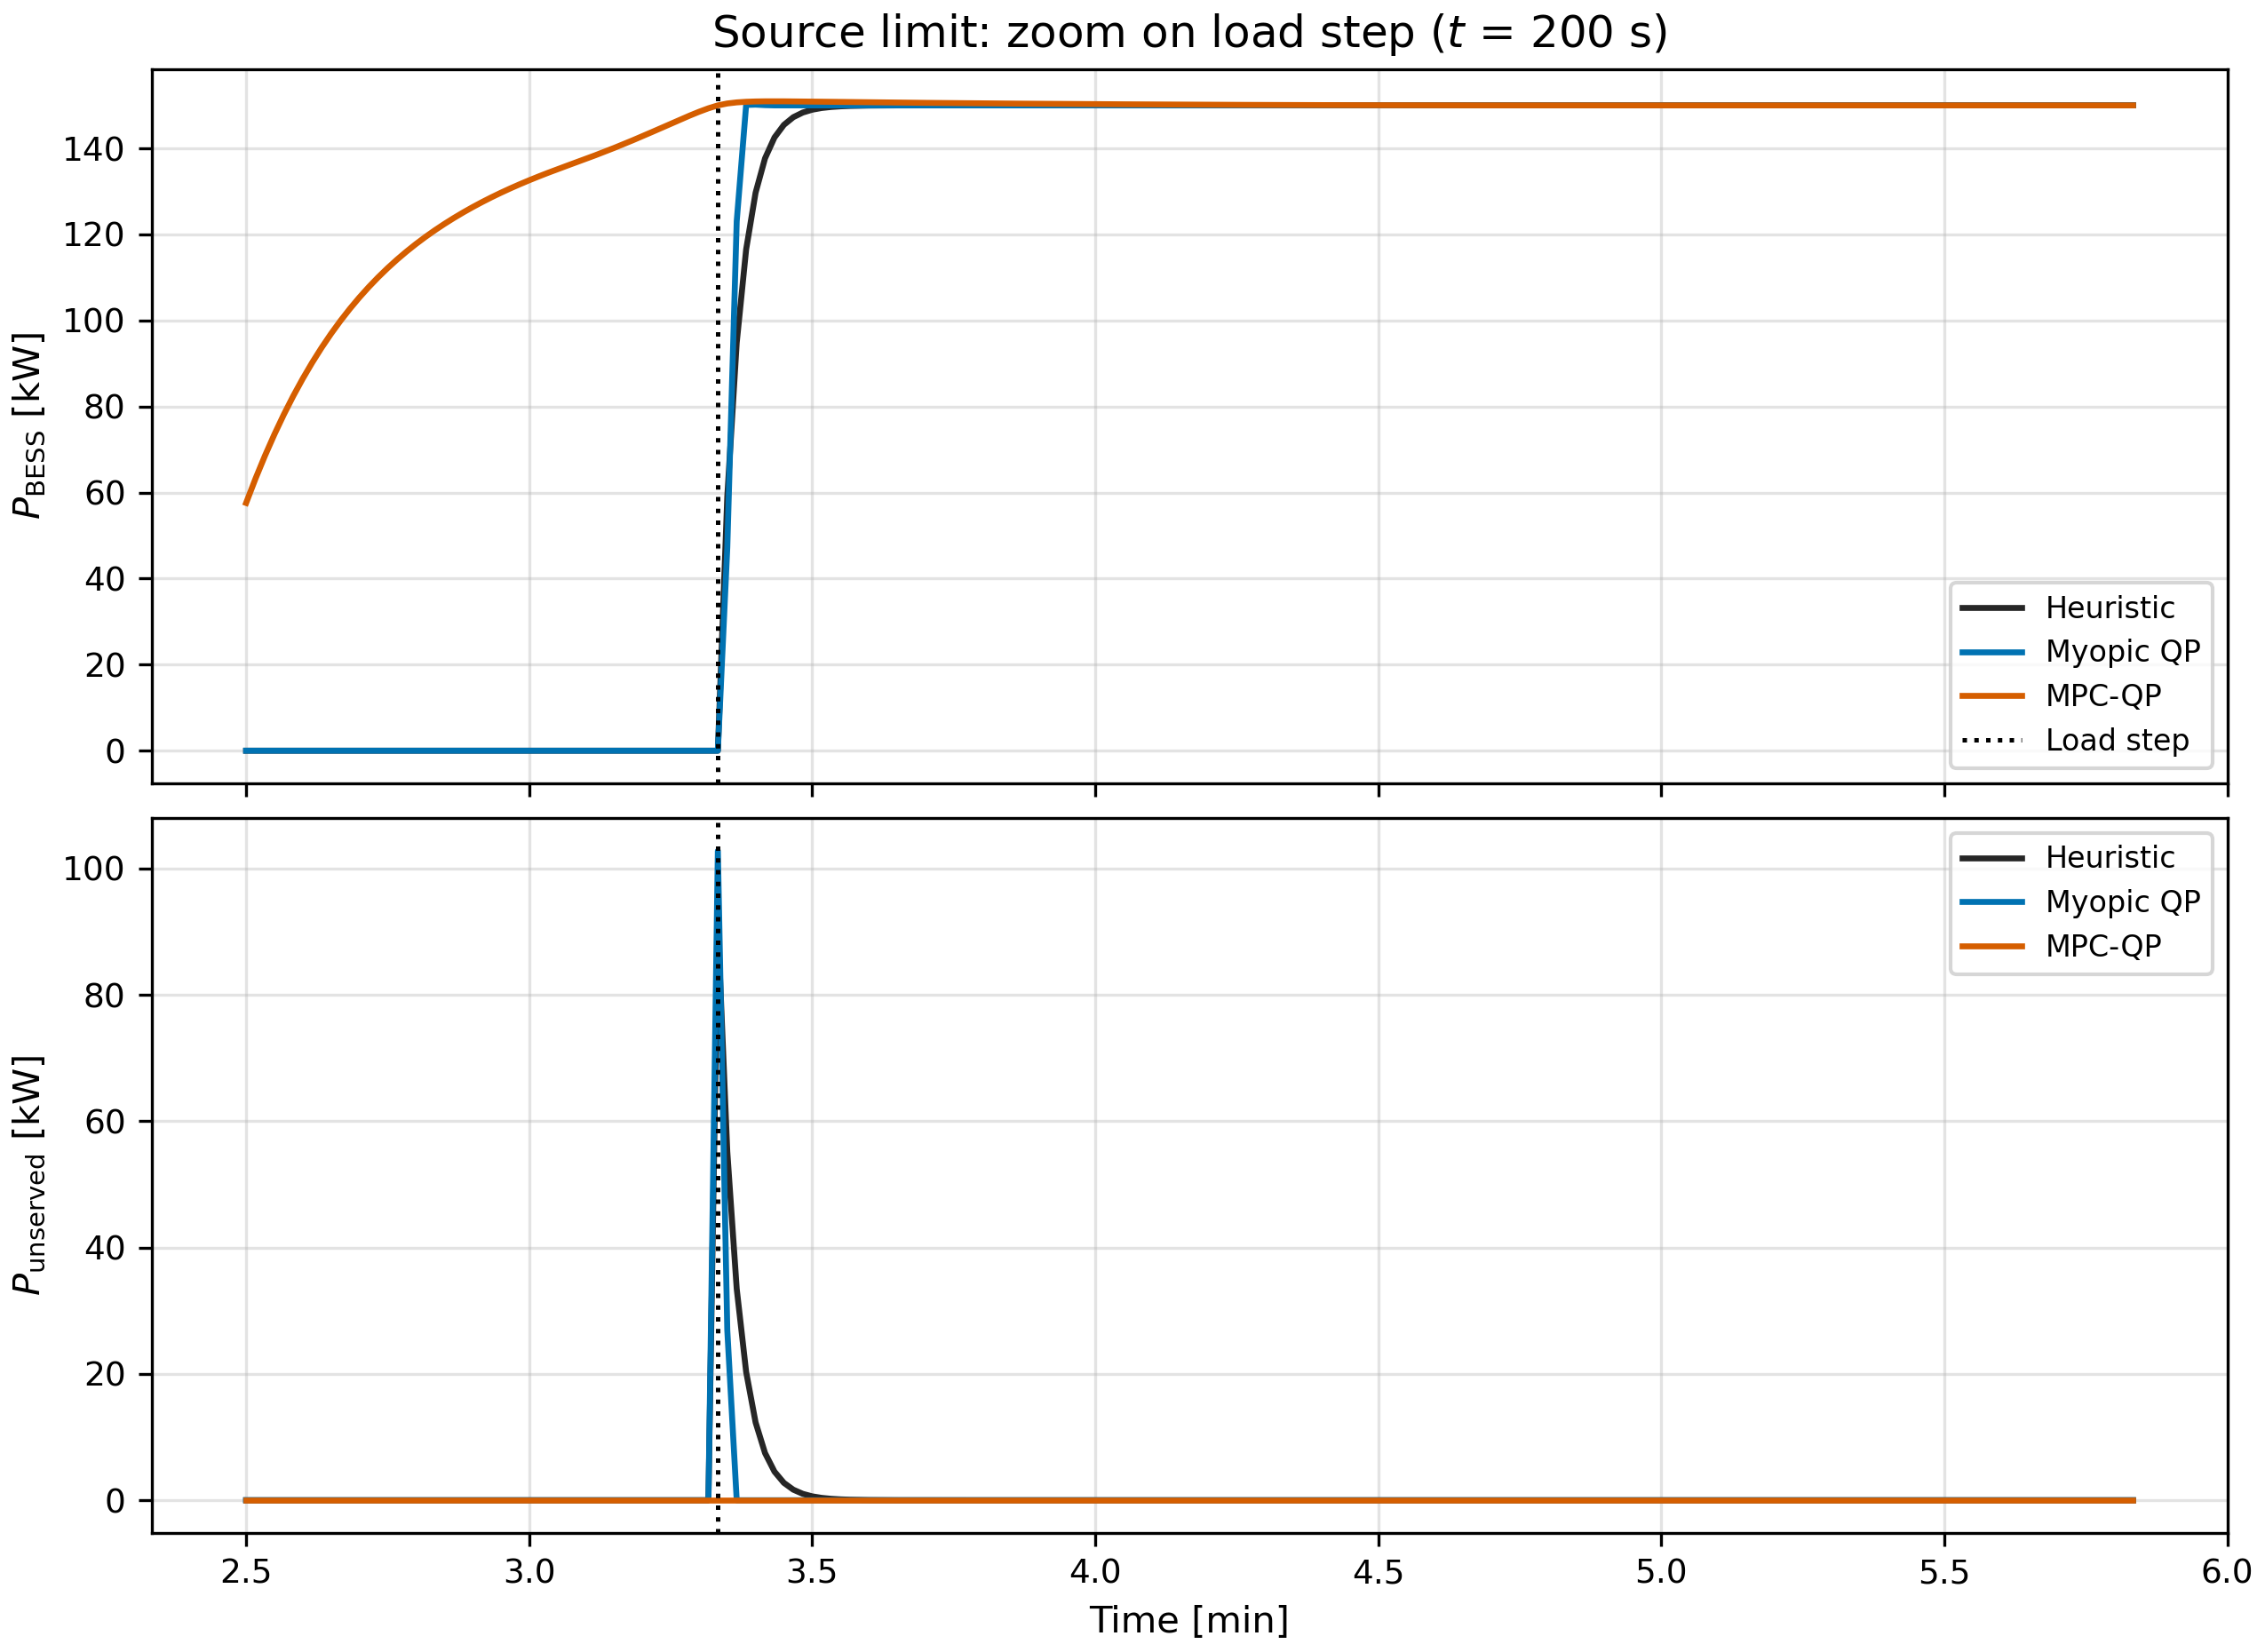
\includegraphics[width=0.85\textwidth]{comp_limite_fonte_zoom_degrau.png}
\caption{Source limit, 11~September campaign: zoom on the $750\to 950$\,kW step. MPC-QP removes $P_{\mathrm{unserved}}$; myopic QP (102.78\,kW) exceeds the heuristic peak (90.98\,kW).}
\label{fig:limit_zoom}
\end{figure*}

Fig.~\ref{fig:loss_zoom} illustrates source loss as complementary analysis (full panels and source-return figures omitted for space; return replicates the same preparation mechanism). With foresight, MPC-QP raises $P_{\mathrm{BESS}}$ before the event, whereas heuristic and myopic QP react only at outage onset. The value here is transient mitigation down to the scenario-specific bound---not elimination of the structural energy deficit.

\begin{figure*}[!t]
\centering
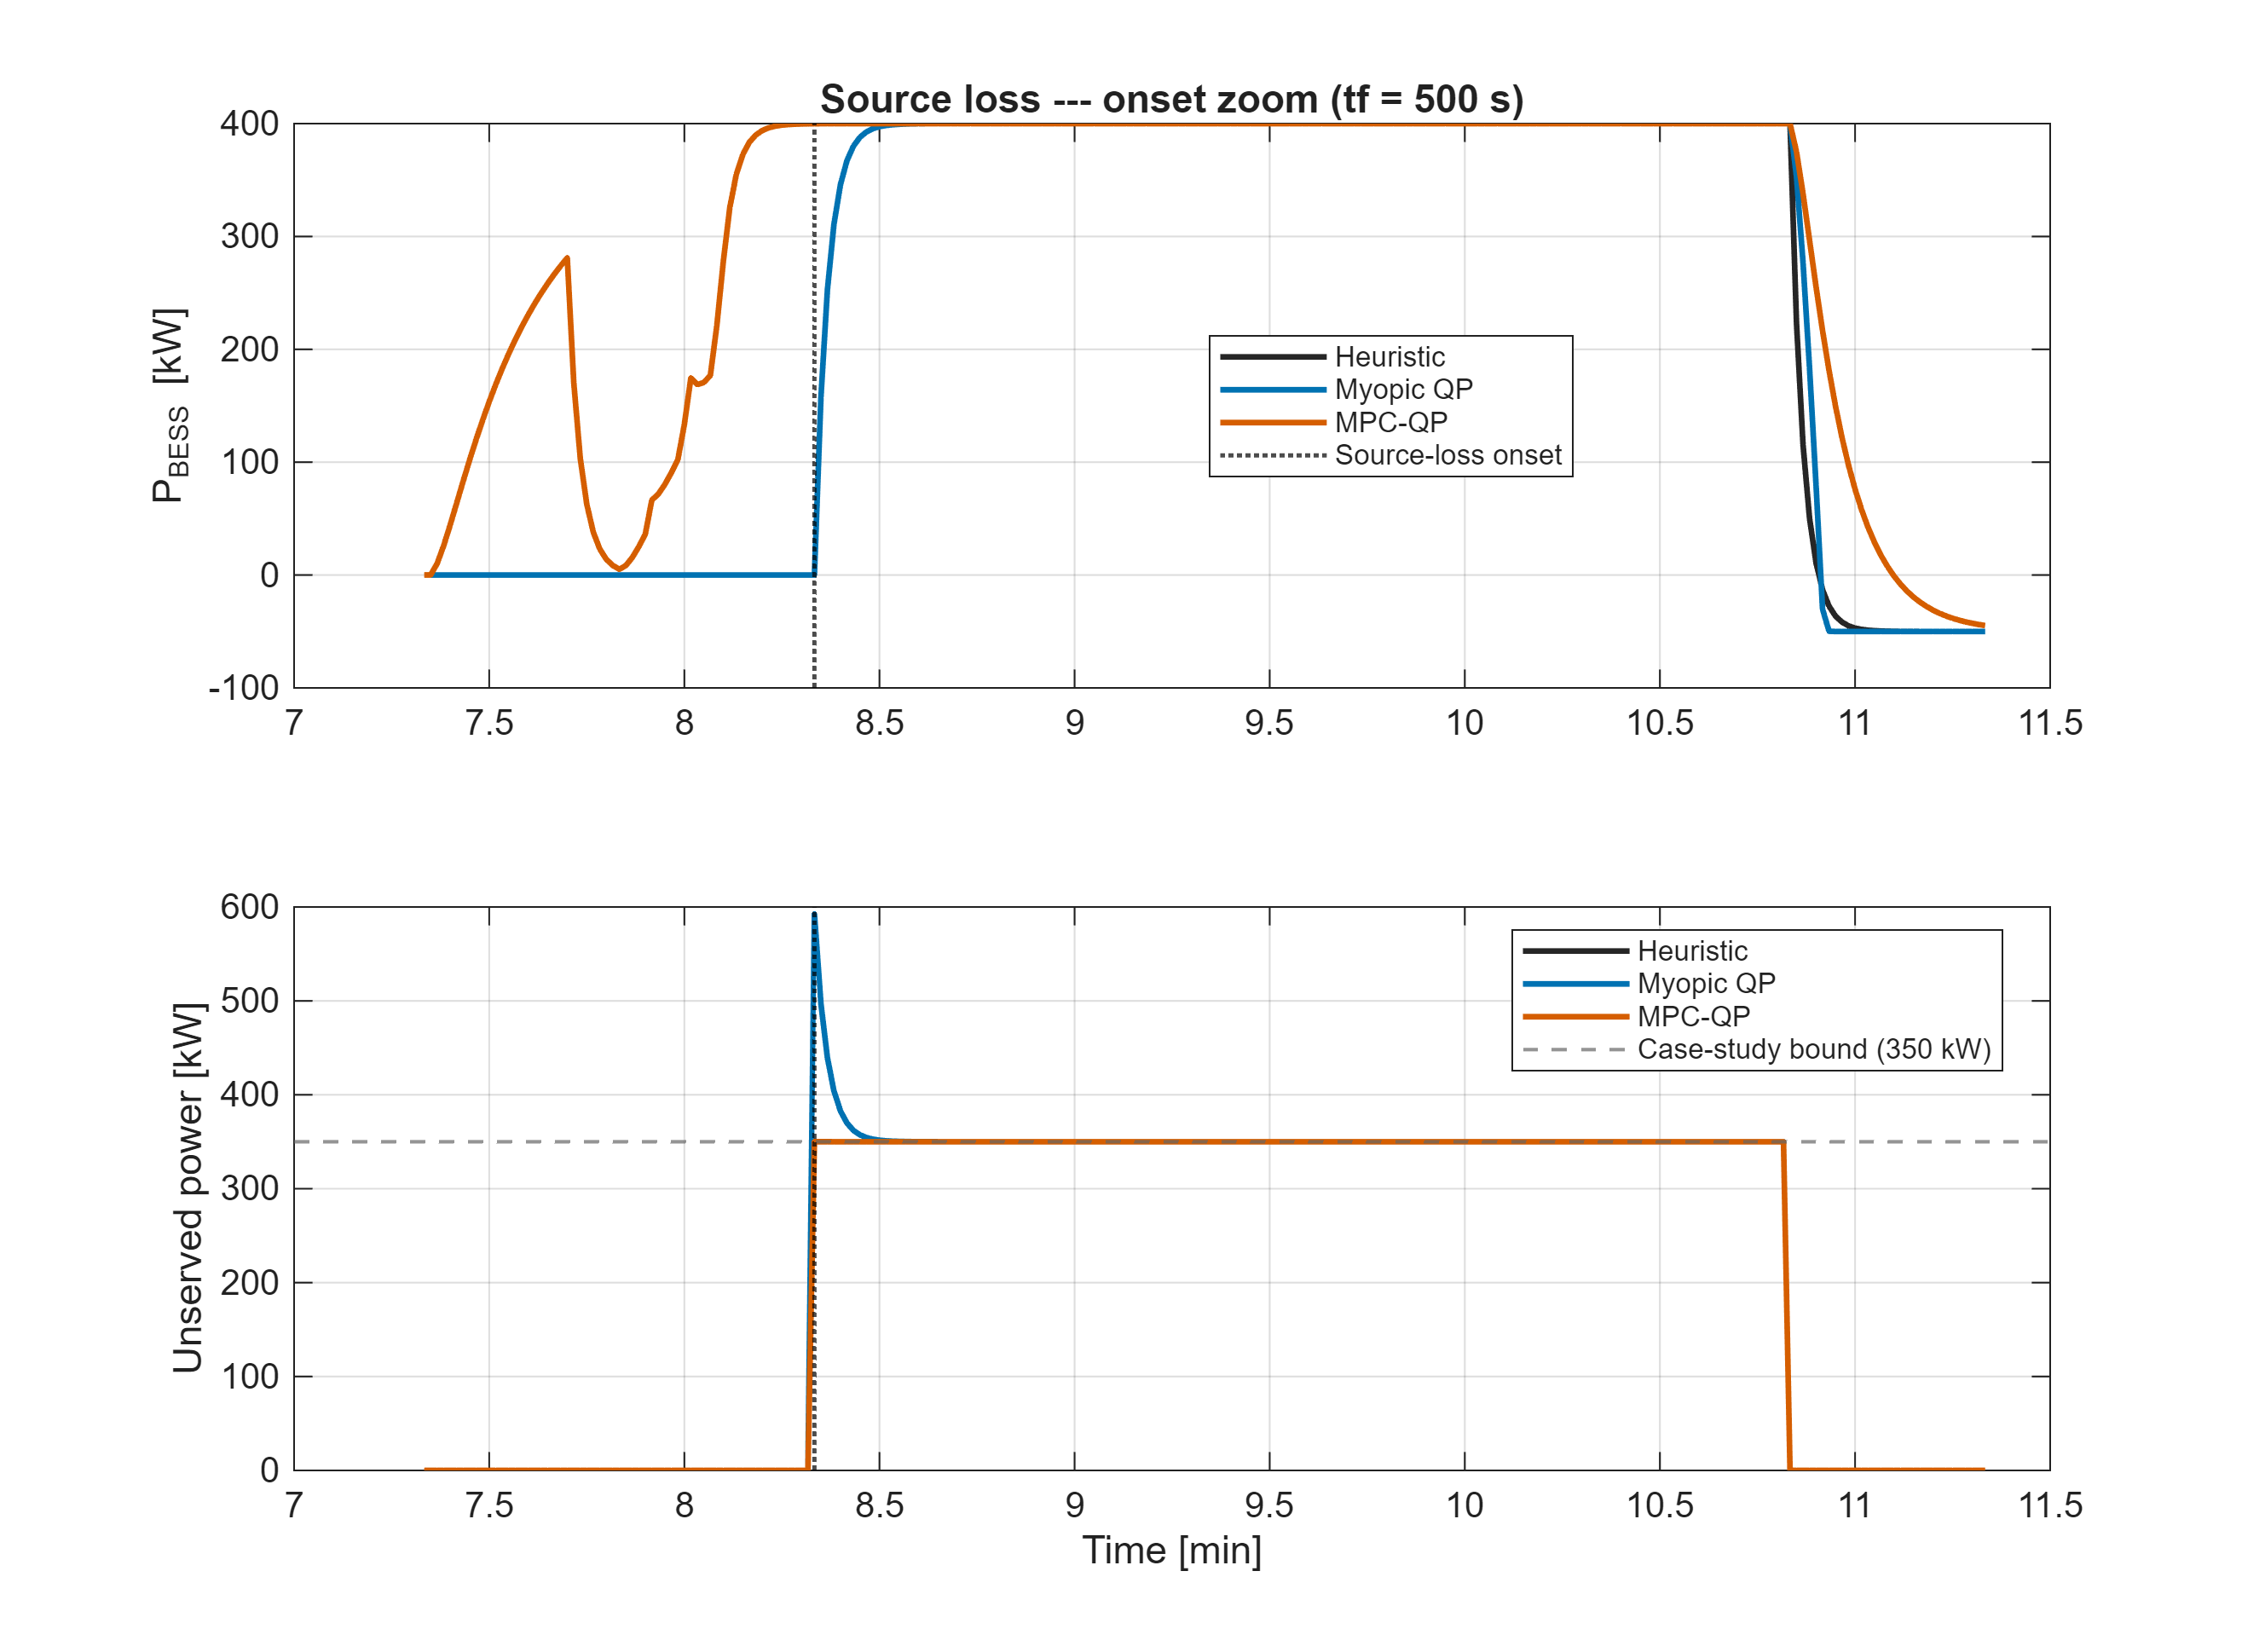
\includegraphics[width=0.85\textwidth]{comp_perda_fonte_zoom_falha.png}
\caption{Source loss, 11~September campaign: zoom of $P_{\mathrm{BESS}}$ and unserved power at fault onset; MPC-QP pre-positions to the $\approx 350$\,kW bound.}
\label{fig:loss_zoom}
\end{figure*}

\subsection{Role of foresight}
To isolate the value of advance information, the source-loss scenario was repeated with the same MPC-QP while masking future events in the horizon (foresight OFF). Results are reported in Table~\ref{tab:foresight}.

\begin{table}[!t]
\centering
\caption{MPC-QP under source loss: foresight ON vs OFF}
\label{tab:foresight}
\footnotesize
\setlength{\tabcolsep}{3.5pt}
\begin{tabular}{@{}lccc@{}}
\toprule
Mode & $P_{\mathrm{un}}^{\max}$ [kW] & $E_{\mathrm{un}}$ [kWh] & SOC$_f$ [\%] \\
\midrule
Foresight ON & 350.07 & 14.58 & 57.10 \\
Foresight OFF & 592.56 & 14.75 & 57.79 \\
\bottomrule
\end{tabular}
\end{table}

Three observations stand out. First, without foresight the peak collapses to the reactive value ($\approx\SI{593}{\kilo\watt}$): the MPC-QP advantage is not intrinsic to QP alone, but to seeing the event with lead time compatible with $\tau_b$ and $N_p$. The OFF case still uses the return-to-normal fill of future $g$ described above. Second, unserved energy changes little (14.58 vs.\ 14.75\,kWh): for a short outage ($\SI{150}{\second}$), total energy deficit is dominated by the bound $P_{\mathrm{load}}-P_{\mathrm{BESS}}^{\max}$ over the contingency; foresight mainly shapes the initial peak. Third, final SOC remains close in both modes, indicating that anticipation consumes a modestly larger share of useful energy before the fault in exchange for reducing the severe $P_{\mathrm{unserved}}$ transient to about \SI{350}{\kilo\watt}. On accepted V5 solutions of the seven principal scenarios, SOC-sign mismatch versus piecewise integration occurs in $100/8353$ steps ($1.20\%$); the worst SOC predictor error among those cases is $0.044$\,pp, with no bound violation of the piecewise reference.

In practice, foresight may come from protection alarms, switching signals, HPC/AI load forecasts or operational schedules---that is, detectable or schedulable events. Without such a signal the controller remains valid, yet behaves as a computationally expensive reactive optimizer. The method does not claim universal robustness to completely random outages.

\subsection{Sensitivity}
Table~\ref{tab:nprep} varies $N_{\mathrm{prep}}\in\{0,10,30,45\}$ with foresight ON. In all cases, $P_{\mathrm{unserved}}^{\max}$ stays near the bound ($\approx\SI{350}{\kilo\watt}$--\SI{350.4}{\kilo\watt}) and unserved energy remains $\approx\SI{14.58}{\kilo\watt\hour}$. The $N_{\mathrm{prep}}=30$ peak $350.08$\,kW in that historical table is \emph{not} the 11~September V5 KPI ($350.07$\,kW in Table~\ref{tab:punserved}). In particular, $N_{\mathrm{prep}}=0$ already reaches $\approx\SI{350.27}{\kilo\watt}$: primary foresight comes from the horizon $N_p$ and the future event constraint~\eqref{eq:event}; $N_{\mathrm{prep}}$ only shapes the pre-event ramp/tracking. Once the event enters $N_p$ and the constraint is active at the outage instant, temporal coupling in the dynamic model induces pre-actuation: the optimizer raises $u$ beforehand to respect first-order dynamics. Thus $N_{\mathrm{prep}}$ is not the key foresight mechanism in this case.

\begin{table}[!t]
\centering
\caption{Sensitivity to $N_{\mathrm{prep}}$ (source loss, foresight ON; \emph{historical} campaign, not re-extracted from the 11~September consolidation)}
\label{tab:nprep}
\begin{tabular}{@{}rccc@{}}
\toprule
$N_{\mathrm{prep}}$ & $P_{\mathrm{unserved}}^{\max}$ [kW] & Unserved energy [kWh] & Mean $t_{\mathrm{QP}}$ [s] \\
\midrule
0 & 350.27 & 14.58 & 0.071 \\
10 & 350.43 & 14.58 & 0.065 \\
30 & 350.08 & 14.58 & 0.060 \\
45 & 350.04 & 14.58 & 0.089 \\
\bottomrule
\end{tabular}
\end{table}

The converter time constant (Table~\ref{tab:tau}) keeps $P_{\mathrm{unserved}}^{\max}$ at the scenario-specific bound for $\tau_b\in\{1,2,4\}$\,s in the 11~September jobs ($350.00$--$350.07$\,kW). Residual fallback is $2.00\%$ ($\tau_b=\SI{1}{\second}$), $1.58\%$ ($\tau_b=\SI{2}{\second}$) and $0.08\%$ ($\tau_b=\SI{4}{\second}$). Ranking among the 11~September controllers is preserved under this first-order $\tau_b$ sweep; that does \emph{not} validate LCL/PLL/UPS dynamics.

\begin{table}[!t]
\centering
\caption{Sensitivity to $\tau_b$ (source loss, foresight ON; 11~September jobs)}
\label{tab:tau}
\begin{tabular}{@{}rccc@{}}
\toprule
$\tau_b$ [s] & $P_{\mathrm{unserved}}^{\max}$ & Energy & FB \\
 & [kW] & [kWh] & [\%] \\
\midrule
1 & 350.00 & 14.58 & 2.00 \\
2 & 350.07 & 14.58 & 1.58 \\
4 & 350.02 & 14.58 & 0.08 \\
\bottomrule
\end{tabular}
\end{table}

\subsection{Prolonged critical outage}
Under an approximately \SI{2}{\hour} outage at constant \SI{750}{\kilo\watt} (outage window $[600,7800)$\,s, $T_f=\SI{9600}{\second}$), heuristic and MPC-QP were compared (Table~\ref{tab:outage}). Both reach $\mathrm{SOC}_{\min}=\SI{20}{\percent}$. After useful BESS depletion, $P_{\mathrm{unserved}}^{\max}=\SI{750}{\kilo\watt}$. Unserved energy is $1309.95$\,kWh (heuristic) vs.\ $1312.33$\,kWh (V5): MPC leaves $\approx 2.38$\,kWh \emph{more} unserved. Time with unmet power equals the $7200$\,s outage because the $400$\,kW rating is below the load. Final SOC $\approx 24.75\%$ / $24.73\%$ is \emph{after} restoration and recharge, not the SOC at $\mathrm{SOC}_{\min}$; pre-event SOC is $60\%$ / $59.50\%$. A $7200$\,s ``recovery'' column is the outage duration until the source returns, not autonomous BESS restoration. Closed-loop generator coordination is not simulated. A later exogenous $400$\,kW injection (package B6; not coordinated dispatch) reduced unserved energy to $513.31$\,kWh (heuristic) versus $538.52$\,kWh (V5): MPC is not automatically better when a genset is an open-loop add-on.

\begin{table}[!t]
\centering
\caption{Prolonged critical outage ($\approx\SI{2}{\hour}$, \SI{750}{\kilo\watt} load)}
\label{tab:outage}
{\footnotesize\setlength{\tabcolsep}{2.8pt}%
\begin{tabular}{@{}lcccc@{}}
\toprule
Control & $P_{\mathrm{un}}^{\max}$ & $E_{\mathrm{un}}$ & SOC$_{\min}$ & SOC$_f$ \\
 & [kW] & [kWh] & [\%] & [\%] \\
\midrule
Heuristic & 750.00 & 1309.95 & 20.00 & 24.75 \\
MPC-QP V5 & 750.00 & 1312.33 & 20.00 & 24.73 \\
\bottomrule
\end{tabular}}
\end{table}

The interpretation is energetic, not merely control-theoretic. Useful energy between $\mathrm{SOC}_{\mathrm{ref}}=\SI{60}{\percent}$ and $\mathrm{SOC}_{\min}=\SI{20}{\percent}$ is approximately
\begin{equation}
E_{\mathrm{useful}}\approx\frac{60-20}{100}\,E_{\mathrm{bat}}\,\eta_{\mathrm{d}}
=\SI{190}{\kilo\watt\hour}.
\end{equation}
Even with continuous discharge at \SI{400}{\kilo\watt}, this reserve covers only tens of minutes of partial support; the minimum instantaneous deficit during full BESS support remains \SI{350}{\kilo\watt}. Thus MPC-QP improves the initial contingency transient (when foresight is adequate), but \emph{cannot create missing energy}: the controller does not invent power or energy beyond the installed BESS rating and stored charge~\cite{zhao2023bess,aghmadi2024ess,zhang2024reliability}. In long outages, performance is dominated by nominal BESS power, available energy and backup sizing; resilience then requires a generator, a second feeder, or a larger energy reservoir rather than a more sophisticated EMS alone. The EMS role in this regime is disciplined reserve management down to $\mathrm{SOC}_{\min}$, avoiding premature depletion and respecting power limits---an objective both controllers meet similarly in the prolonged-outage simulation.

\subsection{Second-event limit test (later package)}
\label{sec:second}
Package B6 (not the 11~September consolidation; $\mathrm{SOC}_0=30\%$, outages $[500,650)$ and $[900,1050)$\,s) is a limit test, not a new official campaign. Table~\ref{tab:second} shows V5 remaining near the $350$\,kW bound ($350.18$\,kW, $4.83\%$ fallback) while the three-scenario competitor hits $750$\,kW, $\mathrm{SOC}_{\min}=20\%$ and $40.01$\,kWh unserved. FF+FB stays at $355.95$\,kW. Sharing $\Delta U$ across scenarios is conservative in Group~A; it is not a guarantee on a depleted second event.

\begin{table}[!t]
\centering
\caption{Second-event limit test (package B6; $\mathrm{SOC}_0=30\%$, two $150$\,s outages)}
\label{tab:second}
{\footnotesize\setlength{\tabcolsep}{2.6pt}%
\begin{tabular}{@{}lcccc@{}}
\toprule
Control & $P_{\mathrm{un}}^{\max}$ & $E_{\mathrm{un}}$ & SOC$_f$ & FB \\
 & [kW] & [kWh] & [\%] & [\%] \\
\midrule
Heuristic & 622.94 & 29.55 & 25.36 & 0 \\
Heur+FS & 362.47 & 29.18 & 24.41 & 0 \\
MPC-QP V5 & 350.18 & 29.17 & 23.71 & 4.83 \\
Stoch.\ 3-sc. & 750.00 & 40.01 & 20.00 & 1.33 \\
FF+FB & 355.95 & 29.18 & 24.20 & 0 \\
\bottomrule
\end{tabular}}
\end{table}

\subsection{Computational aspects}
From the 11~September CSV of the main comparison (MATLAB R2025b, Windows PC, Intel Core i7-4510U, \texttt{quadprog}/\texttt{interior-point-convex}), Table~\ref{tab:tqp} reports \emph{median} and \emph{max} $t_{\mathrm{QP}}$ (\texttt{qp\_p50}/\texttt{qp\_max}), not a mixed-campaign mean. Wall-clock simulation time is larger because it includes plant updates and logging, not only the QP. The reported solve times therefore \emph{do not} demonstrate strict real-time operation at $T_s=\SI{1}{\second}$ on this conventional PC: occasional solves approach a non-negligible fraction of the sampling period, and deployment must budget computational headroom. Cycle time (assembly$+$QP$+$logging) must be reported separately from $t_{\mathrm{QP}}$. On the main V5 load-band job, cycle p50/p95/max $\approx 0.022/0.031/0.242$\,s with Hessian condition $\approx 3.3\times 10^{5}$; QP max on that job is $0.089$\,s, not $0.322$\,s. Deterministic V5 recorded no $T_s$ overruns in the principal short cases; the stochastic competitor recorded three first-sample overruns in its campaign and those are not hidden. The DE2-115 timings are in Section~\ref{sec:embedded}; they are not interchangeable with the i7 numbers. Warm-start speed-up is not claimed.

\begin{table}[!t]
\centering
\caption{MPC-QP $t_{\mathrm{QP}}$ median/max and fallback (11~September CSV)}
\label{tab:tqp}
\begin{tabular}{@{}lccc@{}}
\toprule
Scenario & Med.\ $t_{\mathrm{QP}}$ [s] & Max $t_{\mathrm{QP}}$ [s] & FB [\%] \\
\midrule
Load bands & 0.017 & 0.089 & 0 \\
Source limit & 0.024 & 0.041 & 0 \\
Source loss & 0.020 & 0.046 & 1.58 \\
Multi-burst & 0.019 & 0.031 & 0 \\
\bottomrule
\end{tabular}
\end{table}

\subsection{Forecast error, Monte Carlo, and limitations}
Under perfect foresight, MPC-QP reaches the case-study bound on source loss ($\approx\SI{350.07}{\kilo\watt}$). Magnitude errors of $\pm 10\%$ and $\pm 20\%$ in the predicted load (Table~\ref{tab:err_mag}) were \emph{tolerable}: the peak remains near that bound ($350.03$--$350.63$\,kW). The $+20\%$ case spends more reserve (SOC$_f=49.03\%$ vs.\ $57.10\%$ at zero error). Timing shift of the predicted outage (Table~\ref{tab:err_time}) is the more sensitive axis, but the historical $\approx\SI{699}{\kilo\watt}$ at $-10$\,s is \emph{not} reproduced by the audited protocol. In the 11~September campaign the deterministic V5 peak at $-10$\,s is $350.00$\,kW---the same bound as the unshifted case---because the current sample remains measured while only the future forecast is shifted. None of the 41 grid points on $[-20,+20]$\,s makes V5 worse than the heuristic $592.61$\,kW. A $+10$\,s delay yields $355.57$\,kW; $+20$\,s yields $511.76$\,kW. For the descriptive criterion $P_{\mathrm{unserved}}^{\max}\le 351$\,kW, V5 passes on $[-20,+4]$\,s; that window is not a pre-registered requirement. An $N_{\mathrm{arm}}{=}8$ confirmation gate did \emph{not} improve the ${+}10$\,s Phase-1 re-run ($628$ vs.\ $363$\,kW ungated) and is not presented as a mitigation. That Phase-1 pair is not the 11~September ${+}10$\,s value $355.57$\,kW in Table~\ref{tab:err_time}. The $699$\,kW figure belongs to a previous campaign/protocol; the difference is not attributed to the stochastic competitor, which the deterministic V5 does not use.

Monte Carlo ($n{=}200$ paired forecast errors on one physical loss): V5 mean/p95/max peaks $359.05/384.82/580.32$\,kW; stochastic $350.01/350.03/350.67$\,kW. Stochastic reduces the peak in 188 pairs, ties 12, and never worsens it beyond \SI{0.001}{\kilo\watt}. Mean difference stochastic$-$V5 $= -9.04$\,kW (bootstrap 95\% CI $[-14.02,-4.79]$); median difference only $-0.16$\,kW---the gain sits in the tail. Mean final SOC $55.00\%$ (V5) vs.\ $48.67\%$ (stochastic) in all 200 pairs. Zero peaks worse than the heuristic in 200 draws is not risk zero: the two-sided 95\% binomial upper bound on that rate is $1.83\%$, conditional on the assumed error law. Drawn delays spanned about $-14$ to $+16$\,s, not the full $\pm 20$\,s clip. False alarm (stochastic): SOC $49.42\%$ vs.\ heuristic $60\%$, both without deficit. Unannounced loss: V5 $\approx 592.56$\,kW. Detection delay: V5 $\approx 749.91$\,kW. Do not confuse forecast with detection.

Overall limitations are consolidated as follows. The study uses an aggregated electrical plant without EMT, inner converter loops, DC-link, transfer switch or electrochemical ageing; $\tau_b$ and $\eta$ were not identified on a field battery. Throughput/EFC are utilization proxies, not lifetime. Public traces are mapped into the case-study band; they are not a private feeder campaign. FIL via HDL Verifier was not the implementation path (the DUT is C on Nios, not generated HDL). UART HIL of the heuristic is complete on four scenarios; firmware reports $t_{\mathrm{us}}=0$ for that law, so the overrun column is not a cycle WCET. UART HIL of ADMM was demonstrated in closed loop until the time-limited Nios IP expired and is not a 1200-step KPI table. SIL with \texttt{backend=matlab\_fpga} is MATLAB/\texttt{quadprog} at $N_p{=}12$, not ADMM~C. The stochastic policy is not ported to the FPGA. Prep/reversal/ageing fields in later packages are not used as paper KPIs.

\begin{table}[!t]
\centering
\caption{Load-forecast magnitude error (source loss, MPC-QP)}
\label{tab:err_mag}
\begin{tabular}{@{}rccc@{}}
\toprule
Error [\%] & $P_{\mathrm{unserved}}^{\max}$ [kW] & Energy [kWh] & FB [\%] \\
\midrule
0 & 350.07 & 14.58 & 1.58 \\
$-10$ & 350.18 & 14.59 & 1.33 \\
$+10$ & 350.63 & 14.58 & 2.17 \\
$-20$ & 350.03 & 14.59 & 0.33 \\
$+20$ & 350.28 & 14.58 & 2.75 \\
\bottomrule
\end{tabular}
\end{table}

\begin{table}[!t]
\centering
\caption{Predicted-outage timing shift (source loss, MPC-QP)}
\label{tab:err_time}
\begin{tabular}{@{}rccc@{}}
\toprule
Shift [s] & $P_{\mathrm{unserved}}^{\max}$ [kW] & Energy [kWh] & FB [\%] \\
\midrule
$-10$ & 350.00 & 14.58 & 1.83 \\
0 & 350.07 & 14.58 & 1.58 \\
$+10$ & 355.57 & 14.59 & 1.92 \\
$+20$ & 511.76 & 14.70 & 1.33 \\
\bottomrule
\end{tabular}
\end{table}

\subsection{Consolidated discussion}
Taken together, the 11~September campaign shows that V5 combines foresight with multi-step constrained optimization against converter dynamics---not QP alone and not Heur+FS alone. The later FF+FB package shows that a non-QP law with the same forecasts already obtains the Group~A zeros, so that combination is sufficient but not uniquely necessary on this plant. The myopic QP does not pre-position the BESS: without a future step in the horizon it remains reactive under $\Delta u$ limits and ramp/SOC penalties, and can therefore perform \emph{worse} than the heuristic on the load step (102.78 vs.\ 90.98\,kW). Heur+FS captures part of the foresight benefit on isolated anticipable events, but does not resolve multi-event trade-offs well (multi-burst peak $60.65$\,kW vs.\ $0$\,kW for MPC-QP). The results support four messages:
\begin{enumerate}
\item under demand steps and source-limit saturation, both V5 and FF+FB drive filtered $P_{\mathrm{unserved}}$ below the reporting threshold; heuristic and myopic QP do not;
\item horizon-$N_p$ anticipation with multi-step optimization explains V5 versus Heur+FS and versus myopic QP; it does not imply that no simpler forecast-using law can match Group~A zeros;
\item under grid contingencies, V5 mitigates the peak down to the scenario-specific bound $P_{\mathrm{load}}-P_{\mathrm{BESS}}^{\max}$ when foresight is adequate and well timed, but cannot overcome storage power/energy limits nor random outages without a cue; the stochastic competitor fails a depleted second-event test;
\item in long outages, autonomy is dominated by energy sizing and backup supply; EMS value concentrates on reserve management and normal variable-load operation.
\end{enumerate}

\section{Embedded Validation: SIL and UART HIL}
\label{sec:embedded}

Nomenclature is frozen as follows. \emph{SIL} using the MATLAB FPGA backend (\texttt{matlab\_fpga}) is a reduced-horizon MATLAB copy ($N_p{=}12$, $N_c{=}4$) of the V5 maps, still solved by \texttt{quadprog} on the PC. It shares the HIL \emph{loop} (plant, metrics, ASCII record layout) but calls the controller in-process: it does \emph{not} transmit or parse UART lines and therefore does not validate the serial protocol. It is \emph{not} ADMM~C and is \emph{not} a board execution of the QP. \emph{UART HIL} is the Nios firmware on a Terasic DE2-115 (Cyclone~IV~E, 50\,MHz, 256\,kB on-chip; Quartus Prime Lite 20.1.1). The FPGA device is EP4CE115F29C7. The plant runs in MATLAB over RS-232 115200\,8N1. That serial path is the protocol evidence. \emph{FIL} would be HDL Verifier over Ethernet; it was not implemented because the controller is C/ADMM on Nios, not an HDL DUT.

Table~\ref{tab:sil} compares heuristic and SIL-MPC against golden V5. SIL-MPC matches V5 on Group~A (filtered 0 vs.\ 0; raw V5 $0.018$\,kW on load bands, $\approx 0$ on the source-limit case) and sits $\approx\SI{1}{\kilo\watt}$ above the 350\,kW bound on source loss ($351.17$ vs.\ $350.07$\,kW). Mean SIL $t_{\mathrm{QP}}$ of $7$--$11$\,ms is MATLAB/\texttt{quadprog} on the PC, not Nios ADMM; the first load-band solve reached $0.517$\,s on the PC (not the FPGA).

\begin{table}[!t]
\centering
\caption{SIL MATLAB/\texttt{quadprog} $N_p{=}12$ vs.\ golden V5 ($P_{\mathrm{unserved}}^{\max}$ [kW]; not ADMM~C; V5 from the 11~September campaign)}
\label{tab:sil}
{\footnotesize
\begin{tabular}{@{}lccc@{}}
\toprule
Scenario & Heur. & SIL MPC ($12/4$) & V5 ($60/15$) \\
\midrule
Load bands & 90.98 & 0.00 & 0.018 \\
Source limit & 90.98 & 0.00 & $\approx 0$ \\
Source loss & 592.61 & 351.17 & 350.07 \\
Source return & 592.61 & 351.17 & 350.09 \\
\bottomrule
\end{tabular}}
\end{table}

UART HIL of the \emph{heuristic} on COM4 reproduced SIL to all reported digits on the four short scenarios ($P_{\mathrm{un}}^{\max}=90.98$ or $592.61$\,kW; wall $\approx 57$\,s; 0 fallback). Firmware writes $t_{\mathrm{us}}=0$ for that law, so the overrun column is not a measured cycle WCET. The four runs completed without a recorded protocol timeout; wall $\approx 57$\,s for 1200 steps is \emph{not} a proof that every cycle met $T_s=\SI{1}{\second}$. That is closed-loop evidence for the protocol and the reactive law on the board, not a WCET certificate. The ADMM firmware was linked into 256\,kB (228\,kB image, 26\,kB stack) by overlaying $H$/$K$ and dropping \texttt{printf}. Closed-loop ADMM UART executed (tens of \texttt{RSP} frames) until (i)~OpenCore Plus halted the time-limited Nios IP after $\approx\SI{1}{\hour}$, and (ii)~each QP exceeded $T_s$ by a large margin in software double on the Nios. A MATLAB row labelled \texttt{serial/mpc} with $P_{\mathrm{un}}^{\max}=90.98$ and $57$\,s wall was a switch-capture error (heuristic still selected) and is discarded. No FIL result is claimed. Cycle-time percentiles of ADMM \emph{on the FPGA} for 1200 steps are therefore not a paper table; this Lite platform demonstrated heuristic UART HIL and ADMM execution, not a 1\,s ADMM EMS and not a measured heuristic WCET.

\section{Data Availability}
\label{sec:data}

Campaign CSVs, job fingerprints, the Nios C/ADMM sources, Qsys Tcl, the UART protocol, and the SIL/HIL logs of the 11~September campaign are mirrored in the GitHub repository \url{https://github.com/raonialderete-eng/ems-mpc-datacenter} (private until acceptance; tag \texttt{v1.0.3-ieee-access-rev}) and at the version DOI \url{https://doi.org/10.5281/zenodo.22837544} (snapshot minted from \texttt{v1.0.2-ieee-access-rev}; a matching deposit of tag \texttt{v1.0.3} is pending). The presently minted Zenodo zip does \emph{not} contain the input MATs required by \texttt{caso\_auditado.m}, nor the A1/B2--B6 source trees and results cited for FF+FB and the second-event test; those remain local pending a matching deposit. A MATLAB row labelled \texttt{serial/mpc} at $90.98$\,kW / $57$\,s wall was a switch-capture error and is not in the HIL CSV. The $\approx 1$\,GB raw DIPLOEE/NVML drop is not redistributed; reconstruction of mapped windows from that drop is an external dependency. MATLAB R2025b and Optimization Toolbox reproduce the desktop campaign; DE2-115 $+$ Quartus 20.1 are required only for UART HIL. SIL must not be cited as a MW installation test, as FPGA ADMM, or as UART-protocol validation.

\section{Conclusion}
\label{sec:conclusion}
This paper presented an applied, comparative EMS for AI/HPC data-center energy management with BESS/UPS, together with a reproducible protocol that isolates forecast versus multi-step optimization. The 11~September campaign reports heuristic, Heur+FS, myopic QP, V5 and a three-scenario stochastic competitor that shares the whole $\Delta U$; a later FF+FB package is labelled separately. In nominal load-variation scenarios, both V5 and FF+FB drive filtered unserved-power peaks below \SI{1}{\kilo\watt}, while heuristic and myopic QP remain in the \SIrange{91}{103}{\kilo\watt} range on load bands and source limit (myopic multi-burst $108.90$\,kW); Heur+FS is intermediate on isolated steps and weaker on multi-burst. Under contingencies, V5 reduces the initial transient to the case-study bound ($\approx\SI{350}{\kilo\watt}$ at \SI{750}{\kilo\watt} load) when foresight timing is adequate---about $40.9\%$ peak cut and $1.16\%$ energy cut versus the heuristic, not elimination of the outage deficit. FF+FB reaches $355.95$\,kW on the same source-loss case. Magnitude forecast errors within $\pm 20\%$ preserve that bound. In the audited timing grid a \SI{10}{\second} early shift remains on the bound; a \SI{20}{\second} late shift raises the peak to $\approx\SI{512}{\kilo\watt}$ while still beating the heuristic. Stochastic MPC compresses the Monte Carlo tail at a systematic SOC cost, and fails a depleted second-event limit test ($750$\,kW). SIL using the MATLAB FPGA backend is MATLAB/\texttt{quadprog} at $N_p{=}12$, not ADMM~C and not UART. UART HIL on DE2-115 closed the heuristic on four short runs without a recorded timeout; firmware $t_{\mathrm{us}}=0$, so cycle WCET is not measured. ADMM on Nios is demonstrated, not timed as a 1\,s product on Cyclone~IV Lite. Battery ageing and replacement cost are out of scope of this load-continuity comparison: $N_{\mathrm{EFC}}$ tracks throughput and is not a lifetime or replacement-cost model; the later \texttt{aging\_proxy} field is a multiple of the same throughput and is not used as a KPI.

The main message is fourfold. First, predictive BESS coordination on this aggregated plant removes converter-limited Group~A transients; MPC-QP is sufficient for that, and FF+FB shows it is not uniquely necessary. Second, under source contingencies the benefit is bounded by installed power/energy and by forecast timing. Third, the method does not replace generators, a second feeder, or larger storage, nor does it validate UPS inner loops. Fourth, embedded evidence supports the controller-on-the-same-model claim, not a facility HIL, not FIL, not UART-protocol SIL, and not FPGA ADMM SIL. Converter, SOC and efficiency parameters were not identified on a field battery. Measurement noise is not injected in the 11~September tables; forty later V5 noise jobs exist in package B6 and are not treated as a validated campaign. Code and CSVs are archived as stated in Section~\ref{sec:data}.

\appendices
\section{Audited QP maps}
\label{sec:appqp}

This appendix transcribes the maps executed by the audited assembler (\texttt{montar\_qp\_auditado.m}); it is not a rewrite of \texttt{controle\_mpc\_qp\_v5.m}. Sampling $T_s=\SI{1}{\second}$. Discharge is positive. Measurement at $k$, command $u_k$, BESS power $p_{k+1}$, then interval balance and $\mathrm{SOC}_{k+1}$. Horizons $N_p=60$, $N_c=15$.

\subsection{Condensed prediction}
The stacked command is $\Delta U=[\Delta u_1,\ldots,\Delta u_{N_c}]^\top$ and $U=\mathbf{1}u_{k-1}+T\Delta U$, where $T_{ij}=1$ for $j\le i$ (and $0$ otherwise). Then
\begin{align}
P&=\Phi p_k+\Gamma U=P^{0}+\Gamma T\Delta U,\\
\Phi_i&=a^{i},\qquad
\Gamma_{ij}=b a^{i-j}\quad (j\le i).
\end{align}
Let $C=\mathrm{tril}(\mathbf{1}\mathbf{1}^\top)$. The SOC linearization selects the branch from the free response $P^{0}$ (previous command held):
\begin{equation}
K_i=\frac{100T_s}{3600E_b}
\begin{cases}
1/\eta_{\mathrm{d}}, & P_i^{0}\ge 0,\\
\eta_{\mathrm{c}}, & P_i^{0}<0,
\end{cases}
\qquad
S=\mathbf{1}s_k-C\,\mathrm{diag}(K)\,P.
\end{equation}
Predicted states are eliminated; they are not extra decision variables. If the solved $P$ changes sign versus $P^{0}$, the predictor need not match piecewise integration---that mismatch is reported in the main text.

\subsection{Decision vector and cost}
\begin{equation}
\begin{aligned}
z&=[\Delta U;\ P_g;\ \xi_L;\ \xi_G;\ \xi_R;\ \xi_E],\\
n_z&=N_c+5N_p=315.
\end{aligned}
\end{equation}
Each auxiliary vector has $N_p$ entries and is nonnegative. With $P_b=950$\,kW, $R_b=100$ (kW per sample, i.e.\ kW/s at $T_s=1$\,s), $s^\star=60\%$ and difference operator $D$,
\begin{equation}
\begin{aligned}
J(z)
&= w_g\big\|(P_g-P_g^\star)/P_b\big\|_2^2
 + w_L\big\|\xi_L/P_b\big\|_2^2 \\
&\quad + w_G\big\|\xi_G/P_b\big\|_2^2
 + w_R\big\|\xi_R/P_b\big\|_2^2 \\
&\quad + w_E\big\|\xi_E/P_b\big\|_2^2 \\
&\quad + w_r\big\|(D P_g-e_1 P_{g,k-1})/R_b\big\|_2^2 \\
&\quad + w_s\big\|(S-\mathbf{1}s^\star)/100\big\|_2^2 \\
&\quad + w_T\bigl((S_{N_p}-s^\star)/100\bigr)^2 \\
&\quad + w_p\big\|P/P_b\big\|_2^2
 + w_u\|\Delta U\|_2^2
 + \tfrac{\varepsilon}{2}\|z\|_2^2.
\end{aligned}
\end{equation}
The term $w_u\|\Delta U\|^2$ is \emph{not} divided by $P_b^2$. Regularization $\varepsilon=10^{-6}$ is added to the Hessian. The solver form is $\min_z \tfrac12 z^\top H z+f^\top z$ subject to $Az\le b_A$, $Ez=d$, $\ell\le z\le h$. For each $w\|Fz+c\|^2$ one accumulates $H\leftarrow H+2w F^\top F$ and $f\leftarrow f+2w F^\top c$.

Normal-mode weights: $w_g=3000$, $w_L=10^9$, $w_G=10^8$, $w_R=10^6$, $w_E=10^9$, $w_r=300$, $w_s=1200$, $w_T=12000$, $w_p=20$, $w_u=50$. Event mode changes $w_r=75$, $w_p=2$, $w_u=5$.

\subsection{Constraints}
For each predicted step $i$:
\begin{align}
P_{g,i}+P_i+\xi_{L,i}&=\widehat L_i,\\
p_{\min}&\le P_i\le p_{\max},\\
s_{\min}&\le S_i\le s_{\max},\\
u_{\min,i}&\le U_i\le p_{\max},\\
-dU_{\max}&\le\Delta U\le dU_{\max},\\
P_{g,i}-\xi_{G,i}&\le\widehat M_i,\qquad P_{g,i}\ge 0,
\end{align}
with
\begin{equation}
u_{\min,i}
=\begin{cases}
0, & \widehat{G}_i=0,\\
p_{\min}, & \widehat{G}_i=1.
\end{cases}
\end{equation}
and $P_{g,i}=0$ if $\widehat{G}_i=0$. Recharge is requested only when the source is up, no armed event occupies the horizon, source headroom exists, and $\mathrm{SOC}<\mathrm{SOC}_{\mathrm{ref}}-\Delta_{\mathrm{SOC}}$ with $\Delta_{\mathrm{SOC}}=0.3$ (percentage points) and $P_{\mathrm{rech}}^{\max}=50$\,kW:
\begin{equation}
P_{\mathrm{rech},i}
=\min\!\big(\widehat M_i-\widehat L_i,\ P_{\mathrm{rech}}^{\max},\ |p_{\min}|\big).
\end{equation}
Then $P_{g,i}^{\min,R}=\widehat L_i+P_{\mathrm{rech},i}$ and $P_{g,i}+\xi_{R,i}\ge P_{g,i}^{\min,R}$; the source reference on that branch is also $\widehat L_i+P_{\mathrm{rech},i}$. If recharge is not requested, $\xi_{R,i}$ is fixed at zero. Event support, when positive: $P_i+\xi_{E,i}\ge q_i$. Otherwise the corresponding slacks are fixed at zero. There is no hard source-ramp inequality; ramp enters only the cost. Command rate is not the physical ramp of $p_k$. SOC inequalities use the tabulated bounds with zero extra margin.

\subsection{Event target and no-preview fill}
The raw target is $v_i=\min(\widehat L_i,400)$ during an outage and $v_i=\min(\max(\widehat L_i-\widehat M_i,0),400)$ with the source up. The first $v_i>0$ is $i_e$; $d_{\mathrm{evt}}$ is the run of $v>0$ from $i_e$. Default arming uses $N_{\mathrm{arm}}=\infty$ and $N_{\mathrm{hold}}=1$: if the event has not already started at the current sample, arm only if $i_e\le N_{\mathrm{arm}}$ and $d_{\mathrm{evt}}\ge N_{\mathrm{hold}}$. If already occurring, the constraint stays armed. If armed, $q_i=v_i$ for $i\ge i_e$; for $d=i_e-i\le 30$, $q_i=(30-d+1)v_{i_e}/30$; else $q_i=0$. If not armed, $q_i=0$. Source reference is zero on outage; $\max(0,\widehat L_i-q_i)$ when support is active; $\widehat M_i$ if load exceeds the limit without support; $\widehat L_i$ otherwise, except the recharge branch above.

When foresight of $g$ is off in the 11~September assembler, future $\widehat G$ and $\widehat M$ are filled as source-available / nominal limit (return-to-normal). Package B2/B6 uses persistence of the measured outage. Both are causal hypotheses, not a field detector.

If $\mathrm{exitflag}\le 0$ or the solution is empty, fallback applies: maximum admissible support on outage, or the heuristic with the limiter. Fallback is part of the closed-loop policy.

\subsection{Three-scenario competitor}
For $s\in\{\mathrm{nominal},\ \mathrm{high\ load},\ \mathrm{early\ event}\}$,
\begin{equation}
\min_{\Delta U,\{y_s\}}
\sum_{s}\pi_s J_s(\Delta U,y_s),
\qquad \pi_s=1/3,
\end{equation}
with a \emph{shared} $\Delta U$ and scenario-specific auxiliaries. There is no future branching. Dimension is $N_c+5N_p n_{\mathrm{unique}}\in\{315,615,915\}$. The entire command sequence is common across scenarios; only $u_k=u_{k-1}+\Delta u_1$ is applied and the unused tail is discarded.

\begin{thebibliography}{00}

\bibitem{rossiter2003mpc}
J.~A. Rossiter, \emph{Model-Based Predictive Control: A Practical Approach}. Boca Raton, FL, USA: CRC Press, 2003.

\bibitem{wang2009mpc}
L.~Wang, \emph{Model Predictive Control System Design and Implementation Using MATLAB}. London, U.K.: Springer, 2009.

\bibitem{camacho2007mpc}
E.~F. Camacho and C.~Bordons, \emph{Model Predictive Control}, 2nd~ed. London, U.K.: Springer, 2007.

\bibitem{parisio2014mpc}
A.~Parisio, E.~Rikos, and L.~Glielmo, ``A model predictive control approach to microgrid operation optimization,'' \emph{IEEE Trans. Control Syst. Technol.}, vol.~22, no.~5, pp.~1813--1827, Sep.~2014, doi: 10.1109/TCST.2013.2295737.

\bibitem{wang2023hierarchical}
K.~Wang \emph{et al.}, ``A hierarchical dispatch strategy of hybrid energy storage system in internet data center with model predictive control,'' \emph{Appl. Energy}, vol.~331, Art.~no.~120414, Feb.~2023, doi: 10.1016/j.apenergy.2022.120414.

\bibitem{nair2020mpc}
U.~R. Nair and R.~Costa-Castell{\'o}, ``A model predictive control-based energy management scheme for hybrid storage system in islanded microgrids,'' \emph{IEEE Access}, vol.~8, pp.~97809--97822, 2020, doi: 10.1109/ACCESS.2020.2996434.

\bibitem{sepehrzad2023mpc}
R.~Sepehrzad, J.~Ghafourian, A.~Hedayatnia, A.~Al-Durra, and M.~H. Khooban, ``Experimental and developed DC microgrid energy management integrated with battery energy storage based on multiple dynamic matrix model predictive control,'' \emph{J. Energy Storage}, vol.~74, Art.~no.~109282, Dec.~2023, doi: 10.1016/j.est.2023.109282.

\bibitem{passino1998fuzzy}
K.~M. Passino and S.~Yurkovich, \emph{Fuzzy Control}. Menlo Park, CA, USA: Addison-Wesley, 1998.

\bibitem{astrom1997computer}
K.~J. {\AA}str{\"o}m and B.~Wittenmark, \emph{Computer-Controlled Systems: Theory and Design}, 3rd~ed. Upper Saddle River, NJ, USA: Prentice Hall, 1997.

\bibitem{noland2024ai}
J.~K. N{\o}land, M.~Hjelmeland, and M.~Korp{\aa}s, ``Will energy-hungry AI create a baseload power demand boom?'' \emph{IEEE Access}, vol.~12, pp.~110353--110360, 2024, doi: 10.1109/ACCESS.2024.3440217.

\bibitem{iea2025electricity}
International Energy Agency, \emph{Electricity 2025: Analysis and Forecast to 2027}. Paris, France: IEA, 2025. [Online]. Available: https://www.iea.org/reports/electricity-2025

\bibitem{ieee2025gridready}
IEEE Standards Association, ``Review of industry efforts and standards of grid readiness for data center deployment,'' IEEE SA Industry Connections, Piscataway, NJ, USA, 29~Jan.~2026.

\bibitem{li2025aiload}
Y.~Li and Y.~R. Li, ``AI load dynamics---A power electronics perspective,'' 2025, arXiv:2502.01647.

\bibitem{mughees2025forecast}
M.~Mughees, Y.~Li, Y.~Chen, and Y.~R. Li, ``Short-term load forecasting for AI-data center,'' in \emph{Proc. IEEE Power Energy Soc. Gen. Meeting (PESGM)}, 2025, pp.~1--5, doi: 10.1109/PESGM52009.2025.11225317.

\bibitem{vercellino2026measurement}
R.~Vercellino \emph{et al.}, ``Measurement of generative AI workload power profiles for whole-facility data center infrastructure planning,'' 2026, arXiv:2604.07345.

\bibitem{paananen2023grid}
J.~Paananen, ``Grid-interactive data centers enabling energy transition: Data center's hidden potential to provide essential grid services of a future power system,'' \emph{IEEE Electrific. Mag.}, vol.~11, no.~3, pp.~26--34, Sep.~2023, doi: 10.1109/MELE.2023.3291195.

\bibitem{alapera2018flexibility}
I.~Alaper{\"a}, S.~Honkapuro, and J.~Paananen, ``Data centers as a source of dynamic flexibility in smart grids,'' \emph{Appl. Energy}, vol.~229, pp.~69--79, Nov.~2018, doi: 10.1016/j.apenergy.2018.07.056.

\bibitem{zhang2025flex}
Y.~Zhang, H.~Tang, H.~Li, and S.~Wang, ``Unlocking the flexibilities of data centers for smart grid services: Optimal dispatch and design of energy storage systems under progressive loading,'' \emph{Energy}, vol.~316, Art.~no.~134511, 2025, doi: 10.1016/j.energy.2025.134511.

\bibitem{cioara2016dr}
T.~Cioara \emph{et al.}, ``Optimized flexibility management enacting data centres participation in smart demand response programs,'' \emph{Future Gener. Comput. Syst.}, vol.~78, pp.~330--342, Jan.~2018, doi: 10.1016/j.future.2016.05.010.

\bibitem{kez2021ffr}
D.~Al~Kez, A.~M. Foley, F.~Ahmed, M.~O'Malley, and S.~M. Muyeen, ``Potential of data centers for fast frequency response services in synchronously isolated power systems,'' \emph{Renew. Sustain. Energy Rev.}, vol.~151, Art.~no.~111547, Nov.~2021, doi: 10.1016/j.rser.2021.111547.

\bibitem{teague2025ups}
T.~Teague, S.~S. Refaat, M.~Farrag, and A.~Karaki, ``A comparative study of UPS batteries for data center applications,'' in \emph{Proc. IEEE 19th Int. Conf. Compat., Power Electron. Power Eng. (CPE-POWERENG)}, 2025, pp.~1--6, doi: 10.1109/CPE-POWERENG63314.2025.11027304.

\bibitem{azizi2026gf}
A.~Azizi \emph{et al.}, ``Strengthening data center operations using grid-forming battery energy storage as a line-interactive uninterruptible power supply,'' \emph{Int. J. Electr. Power Energy Syst.}, vol.~175, Art.~no.~111638, 2026, doi: 10.1016/j.ijepes.2026.111638.

\bibitem{zhang2024reliability}
S.~Zhang, C.~Xu, J.~Jiang, and J.~Guo, ``Reliability and economic evaluation of energy storage as backup and load regulation power supply in data centers,'' \emph{Energy Sci. Eng.}, vol.~12, no.~10, pp.~4101--4115, Oct.~2024, doi: 10.1002/ese3.1865.

\bibitem{iqbal2026reliability}
H.~Iqbal and A.~I. Sarwat, ``Reliability-constrained behind-the-meter BESS dispatch for data centers: Co-optimizing utility costs and critical-load continuity under stochastic outages,'' \emph{IEEE Access}, vol.~14, pp.~79227--79252, 2026, doi: 10.1109/ACCESS.2026.3696227.

\bibitem{mou2026stochastic}
G.~Mou, J.~Wang, D.~Cai, and D.~Wu, ``Stochastic dispatch of battery storage via neural policies for AI-driven data centers,'' \emph{IEEE Trans. Ind. Appl.}, early access, 2026, doi: 10.1109/TIA.2026.3677229.

\bibitem{zhao2023bess}
C.~Zhao, P.~B. Andersen, C.~Tr{\ae}holt, and S.~Hashemi, ``Grid-connected battery energy storage system: A review on application and integration,'' \emph{Renew. Sustain. Energy Rev.}, vol.~182, Art.~no.~113400, Aug.~2023, doi: 10.1016/j.rser.2023.113400.

\bibitem{aghmadi2024ess}
A.~Aghmadi and O.~A. Mohammed, ``Energy storage systems: Technologies and high-power applications,'' \emph{Batteries}, vol.~10, no.~4, Art.~no.~141, Apr.~2024, doi: 10.3390/batteries10040141.

\end{thebibliography}

% Author biography (required by IEEE Access; after references, before \EOD).
% No author photograph in the manuscript (photo already provided in the Author Portal).
\begin{IEEEbiographynophoto}{Raoni Alderete}
Raoni Alderete received the B.S.\ degree in electrical engineering from the Universidade Federal de Mato Grosso do Sul (UFMS), Campo Grande, MS, Brazil, in 2013. He is currently pursuing the M.Sc.\ degree in electrical engineering at UFMS. From 2016 to 2020, he was an electrical engineer with Energisa Mato Grosso do Sul, working on distribution construction and maintenance planning. Since 2020, he has been the Founder and Technical Director of MR Energy, Campo Grande, Brazil, where he leads electrical engineering projects involving low- and medium-voltage systems, substations, photovoltaic generation, generators, and uninterruptible power supplies (UPS) for public and private critical facilities. His research interests include model predictive control, battery energy storage systems (BESS), energy management systems for artificial intelligence and high-performance computing (AI/HPC) data centers, and applied optimization for power systems.
\end{IEEEbiographynophoto}

\EOD

\end{document}
